\documentclass[
	numbers=noenddot, % ¬ .e am Ende von TOC
	toc=flat, %Flache TOC
	12pt, % Schriftgröße 
	titlepage, % es wird eine Titelseite verwendet 
	listof=totoc, % Verzeichnisse im Inhaltsverzeichnis aufführen 
	bibliography=totoc, % Literaturverzeichnis im Inhaltsverzeichnis aufführen 
	a4paper
]{scrartcl}

\usepackage[ngerman]{babel}
\usepackage[utf8]{inputenc}
\usepackage[left=2.5cm,right=2.5cm, top=2cm, bottom=2cm]{geometry}
\usepackage{setspace}
\setlength{\footskip}{1.2cm}  % distance between footer and content
\usepackage[toc,page]{appendix} % Anhang
\renewcommand{\appendixname}{Anhang}
\renewcommand{\appendixpagename}{\appendixname} 
\renewcommand{\appendixtocname}{\appendixname} 

% Document variables
\newcommand{\versiondate}{\today}
\newcommand{\firstAuthor}{Oliver Friedrich}
\newcommand{\secondAuthor}{Johannes Hamfler}
\newcommand{\Authors}{\firstAuthor, \secondAuthor}
\newcommand{\shortAuthors}{O. Friedrich, J. Hamfler}
\newcommand{\Title}{Prototypische Umsetzung eines Chatbots zur Terminverwaltung}
\newcommand{\Subtitle}{Masterprojekt WS 2017}
\newcommand{\Supervisor}{Prof. Dr. rer. nat. habil. Michael Frank}
\newcommand{\Affil}{Hochschule für Technik, Wirtschaft und Kultur Leipzig}
\newcommand{\Faculty}{Fakultät Informatik, Mathematik und Naturwissenschaften}
\newcommand{\unterschriftenfelder}[4]{%
  \parbox{\textwidth}{
    \centering #1, \versiondate\\
    \vspace{2cm}
    
    \parbox{6cm}{
      \centering
      \rule{6cm}{1pt}\\
       #2 
    }
    \hfill
    \parbox{6cm}{
      \centering
      \rule{6cm}{1pt}\\
      #3
    }
  }
}

\usepackage[hidelinks]{hyperref}
\hypersetup{%
    pdftitle={\Title},%
    pdfauthor={\Authors},%
    pdfsubject={\Subtitle},%
}

\usepackage[
    headsepline,%
    footsepline,%
    automark,%
]{scrlayer-scrpage}

\usepackage{xcolor}
% % % % color definitions % % % % 
\definecolor{mylightgreen}{HTML}{DFECCF}
\definecolor{mydarkgreen}{HTML}{95C990}
\definecolor{dkgreen}{rgb}{0,0.6,0}
\definecolor{gray}{rgb}{0.5,0.5,0.5}
\definecolor{lightgray}{gray}{0.5}
\definecolor{mauve}{rgb}{0.58,0,0.82}
\definecolor{darkgray}{rgb}{0.4,0.4,0.4}
\definecolor{purple}{rgb}{0.65, 0.12, 0.82}
\definecolor{orange}{rgb}{1, 0.3, 0}

\usepackage{listings}
\lstset{
  backgroundcolor=\color{white},   % choose the background color; you must add \usepackage{color} or \usepackage{xcolor}
  basicstyle=\footnotesize\ttfamily, % the size of the fonts that are used for the code
  breakatwhitespace=false,         % sets if automatic breaks should only happen at whitespace
  breaklines=true,                 % sets automatic line breaking
  captionpos=b,                    % sets the caption-position to bottom
  commentstyle=\color{dkgreen},    % comment style
  deletekeywords={...},            % if you want to delete keywords from the given language
  escapeinside={\%*}{*)},          % if you want to add LaTeX within your code
  extendedchars=true,              % lets you use non-ASCII characters; for 8-bits encodings only, does not work with UTF-8
  frame=single,                    % adds a frame around the code
  keepspaces=true,                 % keeps spaces in text, useful for keeping indentation of code (possibly needs columns=flexible)
  keywordstyle=\color{blue},       % keyword style
  morekeywords={*,...},            % if you want to add more keywords to the set
  numbers=left,                    % where to put the line-numbers; possible values are (none, left, right)
  numbersep=5pt,                   % how far the line-numbers are from the code
  numberstyle=\tiny\color{darkgray}, % the style that is used for the line-numbers
  rulecolor=\color{black},         % if not set, the frame-color may be changed on line-breaks within not-black text (e.g. comments (green here))
  showspaces=false,                % show spaces everywhere adding particular underscores; it overrides 'showstringspaces'
  showstringspaces=false,          % underline spaces within strings only
  showtabs=false,                  % show tabs within strings adding particular underscores
  stepnumber=1,                    % the step between two line-numbers. If it's 1, each line will be numbered
  stringstyle=\color{mauve},	   % string literal style
  tabsize=2,                       % sets default tabsize to 2 spaces
  title=\lstname,                  % show the filename of files included with \lstinputlisting; also try caption instead of title
}


% yaml
\newcommand\YAMLcolonstyle{\color{red}\footnotesize\ttfamily}
\newcommand\YAMLkeystyle{\color{black}\footnotesize\ttfamily}
\newcommand\YAMLvaluestyle{\color{blue}\footnotesize\ttfamily}
\makeatletter
% here is a macro expanding to the name of the language
% (handy if you decide to change it further down the road)
\newcommand\language@yaml{yaml}
\expandafter\expandafter\expandafter\lstdefinelanguage
\expandafter{\language@yaml}
{
  keywords={true,false,null,y,n},
  keywordstyle=\color{darkgray}\ttfamily,
  basicstyle=\YAMLkeystyle,       % assuming a key comes first
  sensitive=false,
  comment=[l]{\#},
  morecomment=[s]{/*}{*/},
  commentstyle=\color{purple}\ttfamily,
  stringstyle=\YAMLvaluestyle\ttfamily,
  moredelim=[l][\color{orange}]{\&},
  moredelim=[l][\color{magenta}]{*},
  moredelim=**[il][\YAMLcolonstyle{:}\YAMLvaluestyle]{:},   % switch to value style at :
  morestring=[b]',
  morestring=[b]",
  literate =    {---}{{\ProcessThreeDashes}}3
                {>}{{\textcolor{red}\textgreater}}1     
                {|}{{\textcolor{red}\textbar}}1 
                {\ -\ }{{\ttfamily\ -\ }}3,
}
% switch to key style at EOL
\lst@AddToHook{EveryLine}{\ifx\lst@language\language@yaml\YAMLkeystyle\fi}
\makeatother
\newcommand\ProcessThreeDashes{\llap{\color{cyan}\ttfamily-{-}-}}


% enable and define SourceCode-Listings
\usepackage{minted}
\setminted{%
    linenos=true,
    breaklines=true,
    tabsize=4,
    numbersep=5pt,
    fontsize=\footnotesize,
}

%\newmintedfile[ansible]{yaml}{}
%\newmintedfile[vagrant]{ruby}{}

\usepackage[babel,german=quotes]{csquotes}

\usepackage[inkscape=force]{svg}
\usepackage{graphicx}
\graphicspath{{./img/}}
\newcommand{\Logo}{\includesvg[height=30px]{img/HTWK-Logo}}
\newcommand{\BigLogo}{\includesvg[height=60px]{img/HTWK-Logo}}

\usepackage{pdfpages}

\usepackage{tabularx}
%\usepackage{fourier} 
%\usepackage{array}
\usepackage{makecell}
%\renewcommand{\cellalign/theadalign}{tl}
\renewcommand\theadalign{tl}
%\renewcommand\theadfont{\bfseries}
\renewcommand\theadgape{\Gape[0pt]}
\renewcommand\cellgape{\Gape[0pt]}
\setcellgapes{0pt}
%\usepackage{cellspace}
%\setlength\cellspacetoplimit{0pt}
%\setlength\cellspacebottomlimit{0pt}


\usepackage[affil-it]{authblk}
\usepackage[colorinlistoftodos,prependcaption,textsize=tiny]{todonotes}
\setlength{\parindent}{0em}

% For folder listings and trees
%\definecolor{folderbg}{RGB}{255,255,255}
%\usepackage{forest}

\usepackage[acronym,toc,shortcuts]{glossaries}
\makeglossaries%

% \newacronym{DNS}{DNS}{Domain Name Service}

\usepackage[
style=alphabetic,
bibstyle=alphabetic,
citestyle=alphabetic,
backend=biber
]{biblatex}
\bibliography{main.bib}

% Enable custom title page
%\titlepage%


\begin{document}


\begin{titlepage}
    \centering
    \textbf{\Huge {\Title}}\\
    \vspace{2cm}
    {\Large \Subtitle}\\
    \vspace{2cm}
    {Betreuer: \Supervisor}\\
    \vspace{1cm}
    {vorgelegt von}\\
    \vspace{0.5cm}
    {\Authors}\\
    \vspace{2cm}
    {\MakeUppercase{\Affil}}\\
    \vspace{0.5cm}
    {\MakeUppercase{\Faculty}}\\
    \vspace{2cm}
    {vorgelegt am:\\ \versiondate}\\
    \vspace{4cm}
    {\BigLogo}
\end{titlepage}


% % % % % % % % % % % % % % % % % % % % % % % % % INHALTSVERZEICHNIS
\chead{}
\ihead{\footnotesize \textsc{\headmark}}
\ohead{}
\ifoot{\Authors}
\cfoot{}
\ofoot{\versiondate}
\pagebreak

\tableofcontents
\pagebreak
% % % % % % % % % % % % % % % % % % % % % % % % % INHALTSVERZEICHNIS

%%%%%% Verzeichnisse %%%%%%
\pagenumbering{gobble}
\listoffigures %Abbildungsverzeichnis
\newpage
\listoftables %Tabellenverzeichnis
\newpage
\renewcommand\lstlistingname{Listing} % Untertitel unter Listing
\renewcommand\lstlistlistingname{Quellcodeverzeichnis} % Verzeichnisname
\def\lstlistingautorefname{Listing} % autoref im text
\lstlistoflistings % Listingverzeichnis
\newpage
\clearpage
%%%%%%%%%%%%%%%%%%%%%%%%%%%
%\listoftodos



% % % % % % % % % % % % % % % % % % % % % % % % % INHALT
\newpage
\pagenumbering{arabic}
\setcounter{page}{1}
\parindent0pt % Keine Absatzeinrückungen
\parskip2ex %Absatzhöhe

\chead{}
\ihead{\footnotesize \textsc{\headmark}}
\ohead{\thepage}
%\automark[subsection]{subsection}
\automark[section]{section}
\ifoot{\Authors}
\cfoot{}
\ofoot{\versiondate}

\section{Einleitung}
\label{einleitung}
Dieses Dokument wurde im Rahmen des Masterprojekts des Studiengangs Informatik an der HTWK-Leipzig erstellt. Es beinhaltet die Entwicklung und prototypische Umsetzung eines Chatbots für die Terminverwaltung des Studentenclubs \glqq Stecker\grqq .

Der Auftrag wurde von der technischen Abteilung des Clubs gestellt. Die Motivation hierfür ist eine einfache, schnelle und zentrale Verwaltung von Schichtplänen, um den Vorstand in der Organisation der Veranstaltungen zu entlasten.
Es wird ein Chatbot benötigt, welcher über die Kommunikationsplattform \glqq Slack\grqq gesteuert werden kann und auch von technisch nicht versierten Mitgliedern bedienbar ist.

Dieses Dokument wird die Anforderungen an den Chatbot präsentieren und bereits vorhandene Lösungen bewerten und gegenüberstellen. Anschließend wird ein Modell für die Verwendung eines Frameworks im Zusammenhang mit Use-Cases erstellt. Weiterhin wird ein Datenbankmodell für die Terminverwaltung entworfen, welches sich nicht nur auf die bekannten Anwendungsfälle beschränken wird. Es wird gesondert auf die praktische Realisierung und die zu beachtenden Probleme bei der Einrichtung eingegangen. Das fertige System wird anschließend Analysiert und Bewertet. Im Schlusswort werden die Autoren das entworfene System den Anforderungen gegenüberstellen und abschließend eine Aussicht für die weitere Entwicklung geben.
% kurz Abstract
% um was gehts, wer gab den auftrag, welcher hintergrund / motivation
% was ist das grobe ziel

\clearpage
\section{Anforderungen und Festlegungen}
\label{anforderungen}
\subsection{Anforderungen des Auftraggebers}
Der Auftraggeber teilt seine Anforderungen in notwendige und optionale Ziele ein, welche nachfolgend aufgelistet werden. Als notwendige Ziele für das Projekt wurden folgende festgelegt.

\begin{itemize}
	\item Chatbot ist in Slack verwendbar
	\item Datenbank, welche Veranstaltungen und Zuweisungen der Mitglieder enthält
	\item Erfassung, welche Mitglieder wie viele Dienste gemacht haben
	\item Abfragefunktion ist für Termine vorhanden
	\item zeitgesteuerte, ereignisbasierte und manuelle Erinnerungsfunktion
	\item Einschränkung der Zielgruppe bzgl. Erinnerungen möglich
	\item einfache Bedienbarkeit
	\item Erweiterbarkeit des Projekts gegeben
	\item MIT-ähnliche Lizenzen für Drittanbietersoftware und -quelltext
	\item Dokumentation der Datenbank
	\item Unabhängigkeit der relevanten Daten vom verwendeten Bot
	\item Zukunftssicherheit
\end{itemize}


Die optionalen Ziele werden nachfolgend aufgeführt.
\begin{itemize}
	\item aus iCal Termine extrahieren
	\item Dienstplan aus Doodle-ähnlicher Umfrage erstellen
	\item Nutzerberechtigungen
	\item Steuerung über E-Mail
	\item containerbasierte Lösung
	\item Caching für schnellere Abfragen
	\item Backup-Strategie
\end{itemize}

% Hier schon das Usecase-Diagramm hin? - NEIN, hier kommt nur das rein, was Ferdi gesagt hat. Alles was wir selbst erarbeitet haben kommt danach.

\subsection{Festlegungen}
% Synonyme, Beschreibungen, Abgrenzungen für die Arbeit

Eine Menge an Terminen wird mit $T$ bezeichnet, Veranstaltungen mit $V$ und Sitzungen mit $S$.

Alle im Rahmen dieser Arbeit erstellten UML-Diagramme entsprechen dem aktuellen UML-Standard, Version 2.5.1. Dieser steht unter \url{https://www.omg.org/spec/UML/2.5.1/} zur Verfügung.

Alle das System nutzenden Akteure werden im Folgenden als Nutzer bezeichnet. Mitarbeiter sind alle Mitarbeiter des Studentenclubs Stecker. Administratoren sind spezielle Nutzer mit zusätzlichen Berechtigungen.
Es bestehen folgende Abhängigkeiten: 

$Nutzer = Administrator \cup Mitarbeiter$ 
%und $Administrator \subset Nutzer$ // unnötig

\subsection{Anwendungsfalldiagramme}

% ??????????? Das klingt eher wie ein Vorwort für den Entwurf der Digaramme. ich würde hier nur Dinge rein schreiben, die sich über mehrere Kapitel erstrecken, so als "globale variablen"
% Ich würde die UML-Usecases schon gern einleiten, wirkt sonst so lieblos, sollen ja auch einen Sinn haben

Die auf den vorherigen Seiten zusammengetragenen obligatorischen Projektziele wurden zur besseren Überprüfung der Ziele in Anwendungsfälle umformuliert. Diese wurden entsprechend \autoref{usecase-auftrag} auf die Akteure \enquote{Bot} und \enquote{Auftraggeber} verteilt.

Die Auftraggeber sind hierbei Ferdinand Malcher und Robert Weisse als Angehörige des Studentenclubs \enquote{Stecker}. Der \enquote{Bot} ist eine nicht näher spezifizierte Chatbot-Technologie, die aber bewusst als Akteur eingeführt wurde, da sie selbständig Aktionen ausführen soll.

\begin{figure}[htbp]
    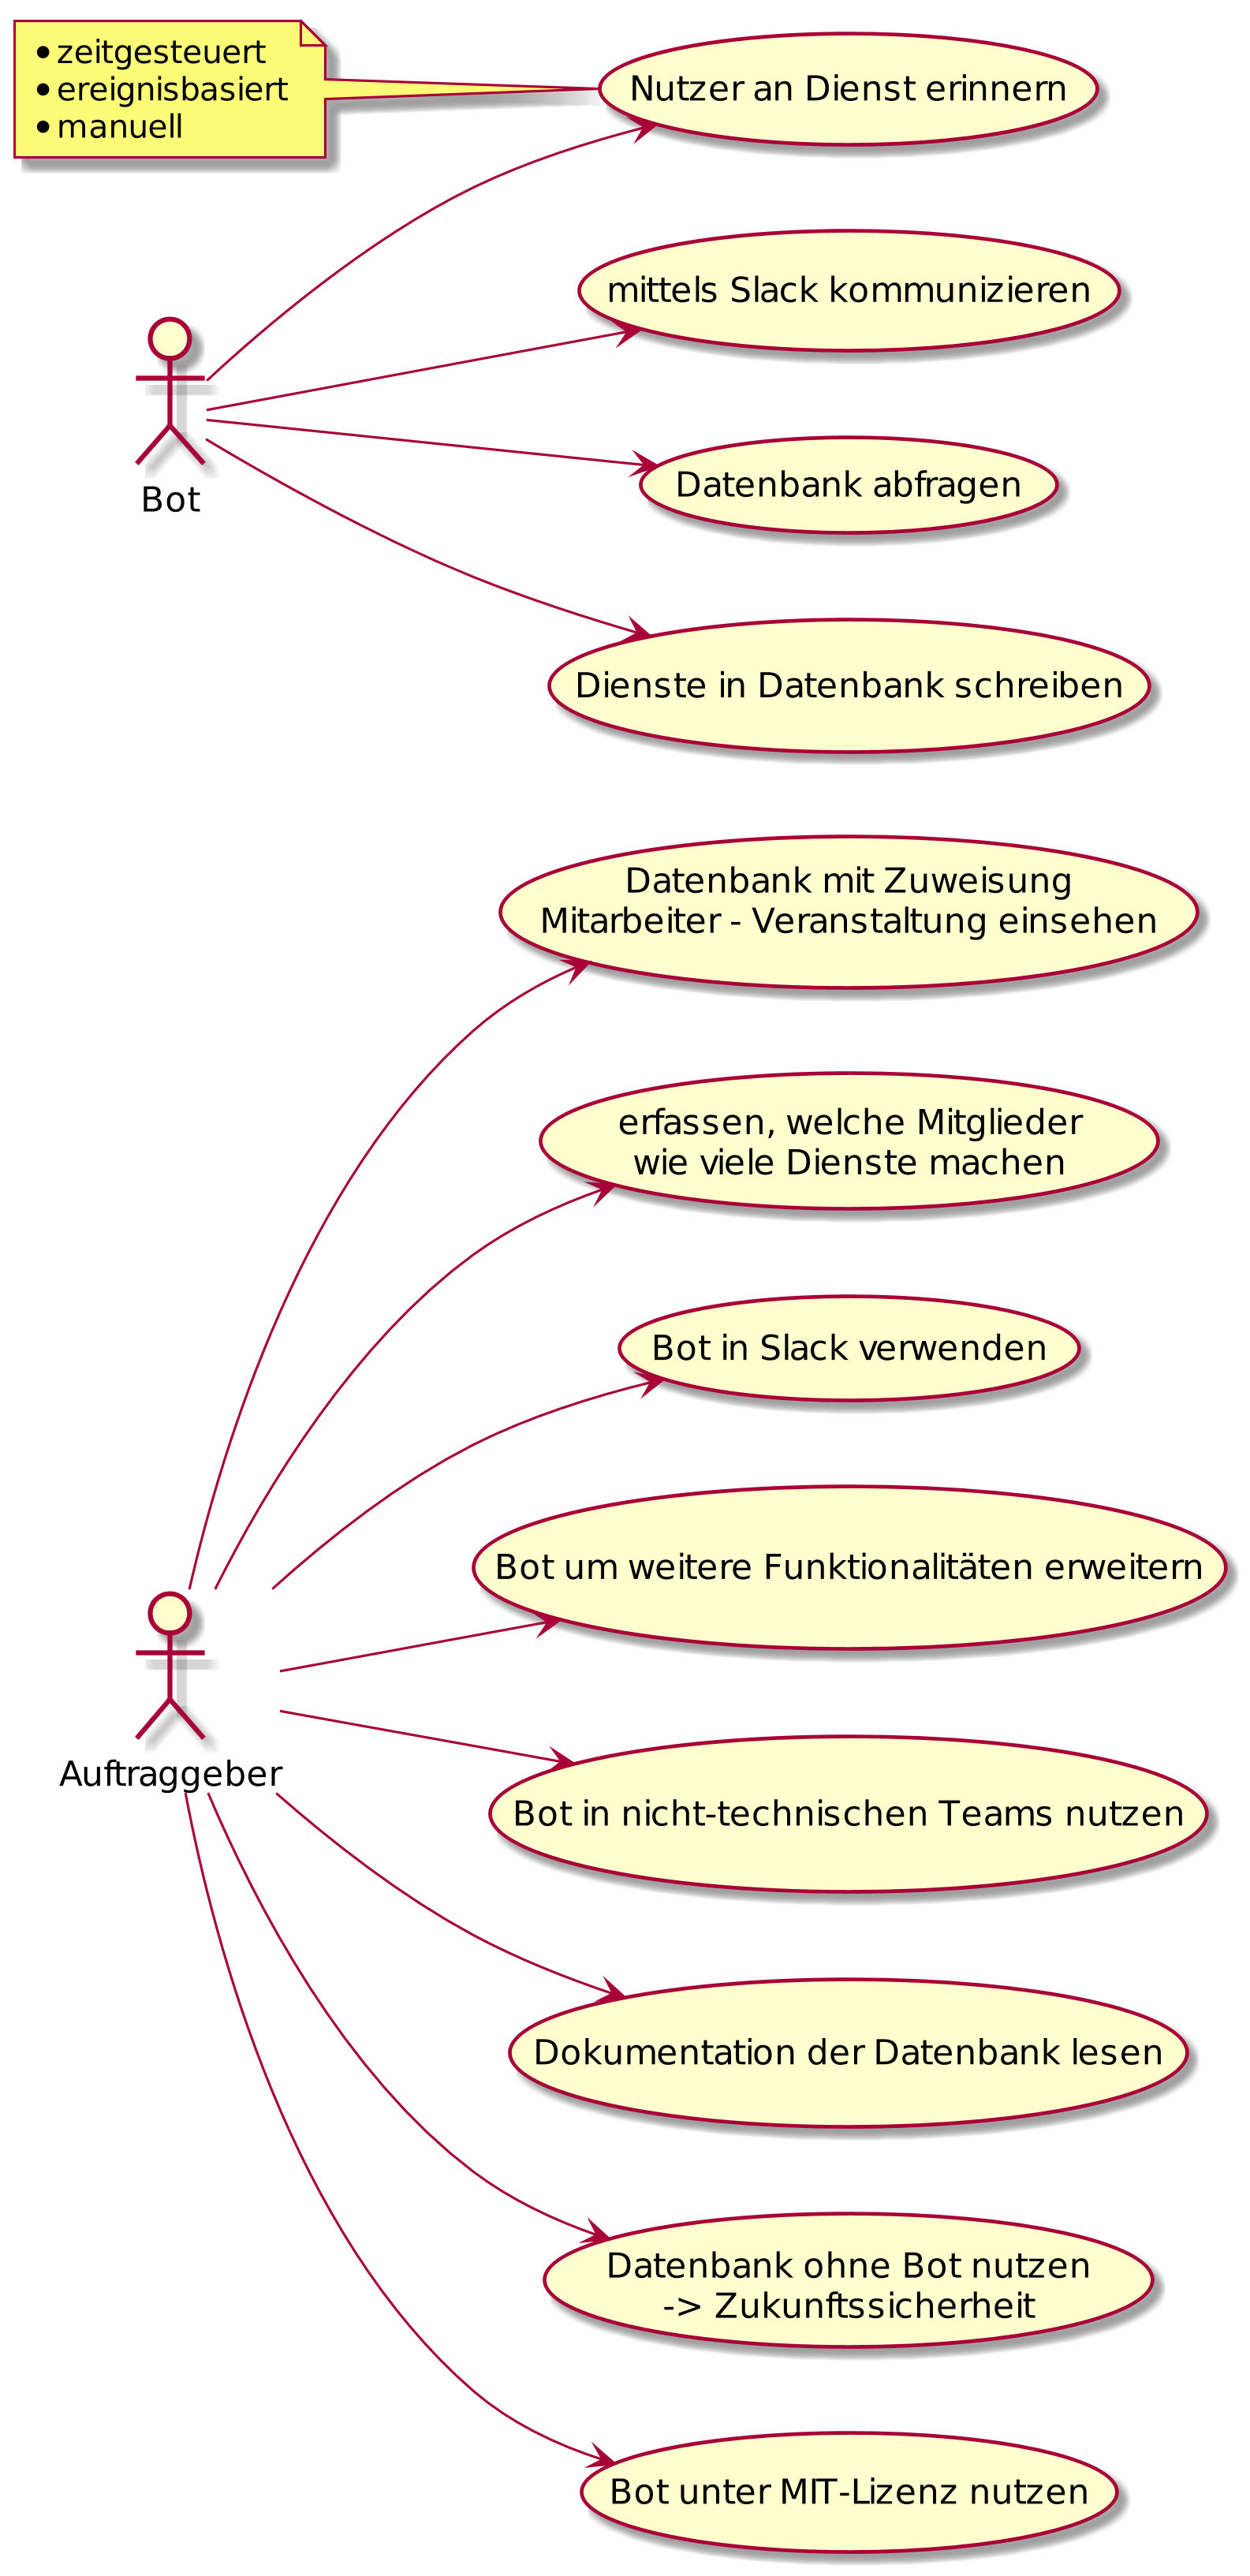
\includegraphics[width=0.7\textwidth]{../docs/uml/usecase-stakeholder.png}
    \caption{Anwendungsfalldiagramm für Auftraggeber und Bot}
    \label{usecase-auftrag}
\end{figure}


Für den zukünftigen Einsatz wurde ein weiteres Anwendungsfalldiagramm zur Unterteilung der Berechtigung der Nutzer erstellt. Gemäß Aufgabenstellung sind in \autoref{img:usecase-berechtigung} die Anwendungsfälle der Nutzer beschrieben. Die darin ebenfalls enthaltene Unterteilung der Berechtigungen dient hier nur der Vollständigkeit, da diese nicht zur initialen Aufgabenstellung gehört.
Eine weitere mögliche Betrachtung ist der unterschiedliche Grad an Fähigkeiten zwischen Administrator und Mitarbeiter. Während es einem Administrator zumutbar ist, beispielweise einen Nutzer direkt per Datenbankzugriff anzulegen, so benötigt der Mitarbeiter eine seinen Fähigkeiten angemessene Schnittstelle wie sie der Chatbot bieten soll.

\begin{figure}[htbp]
    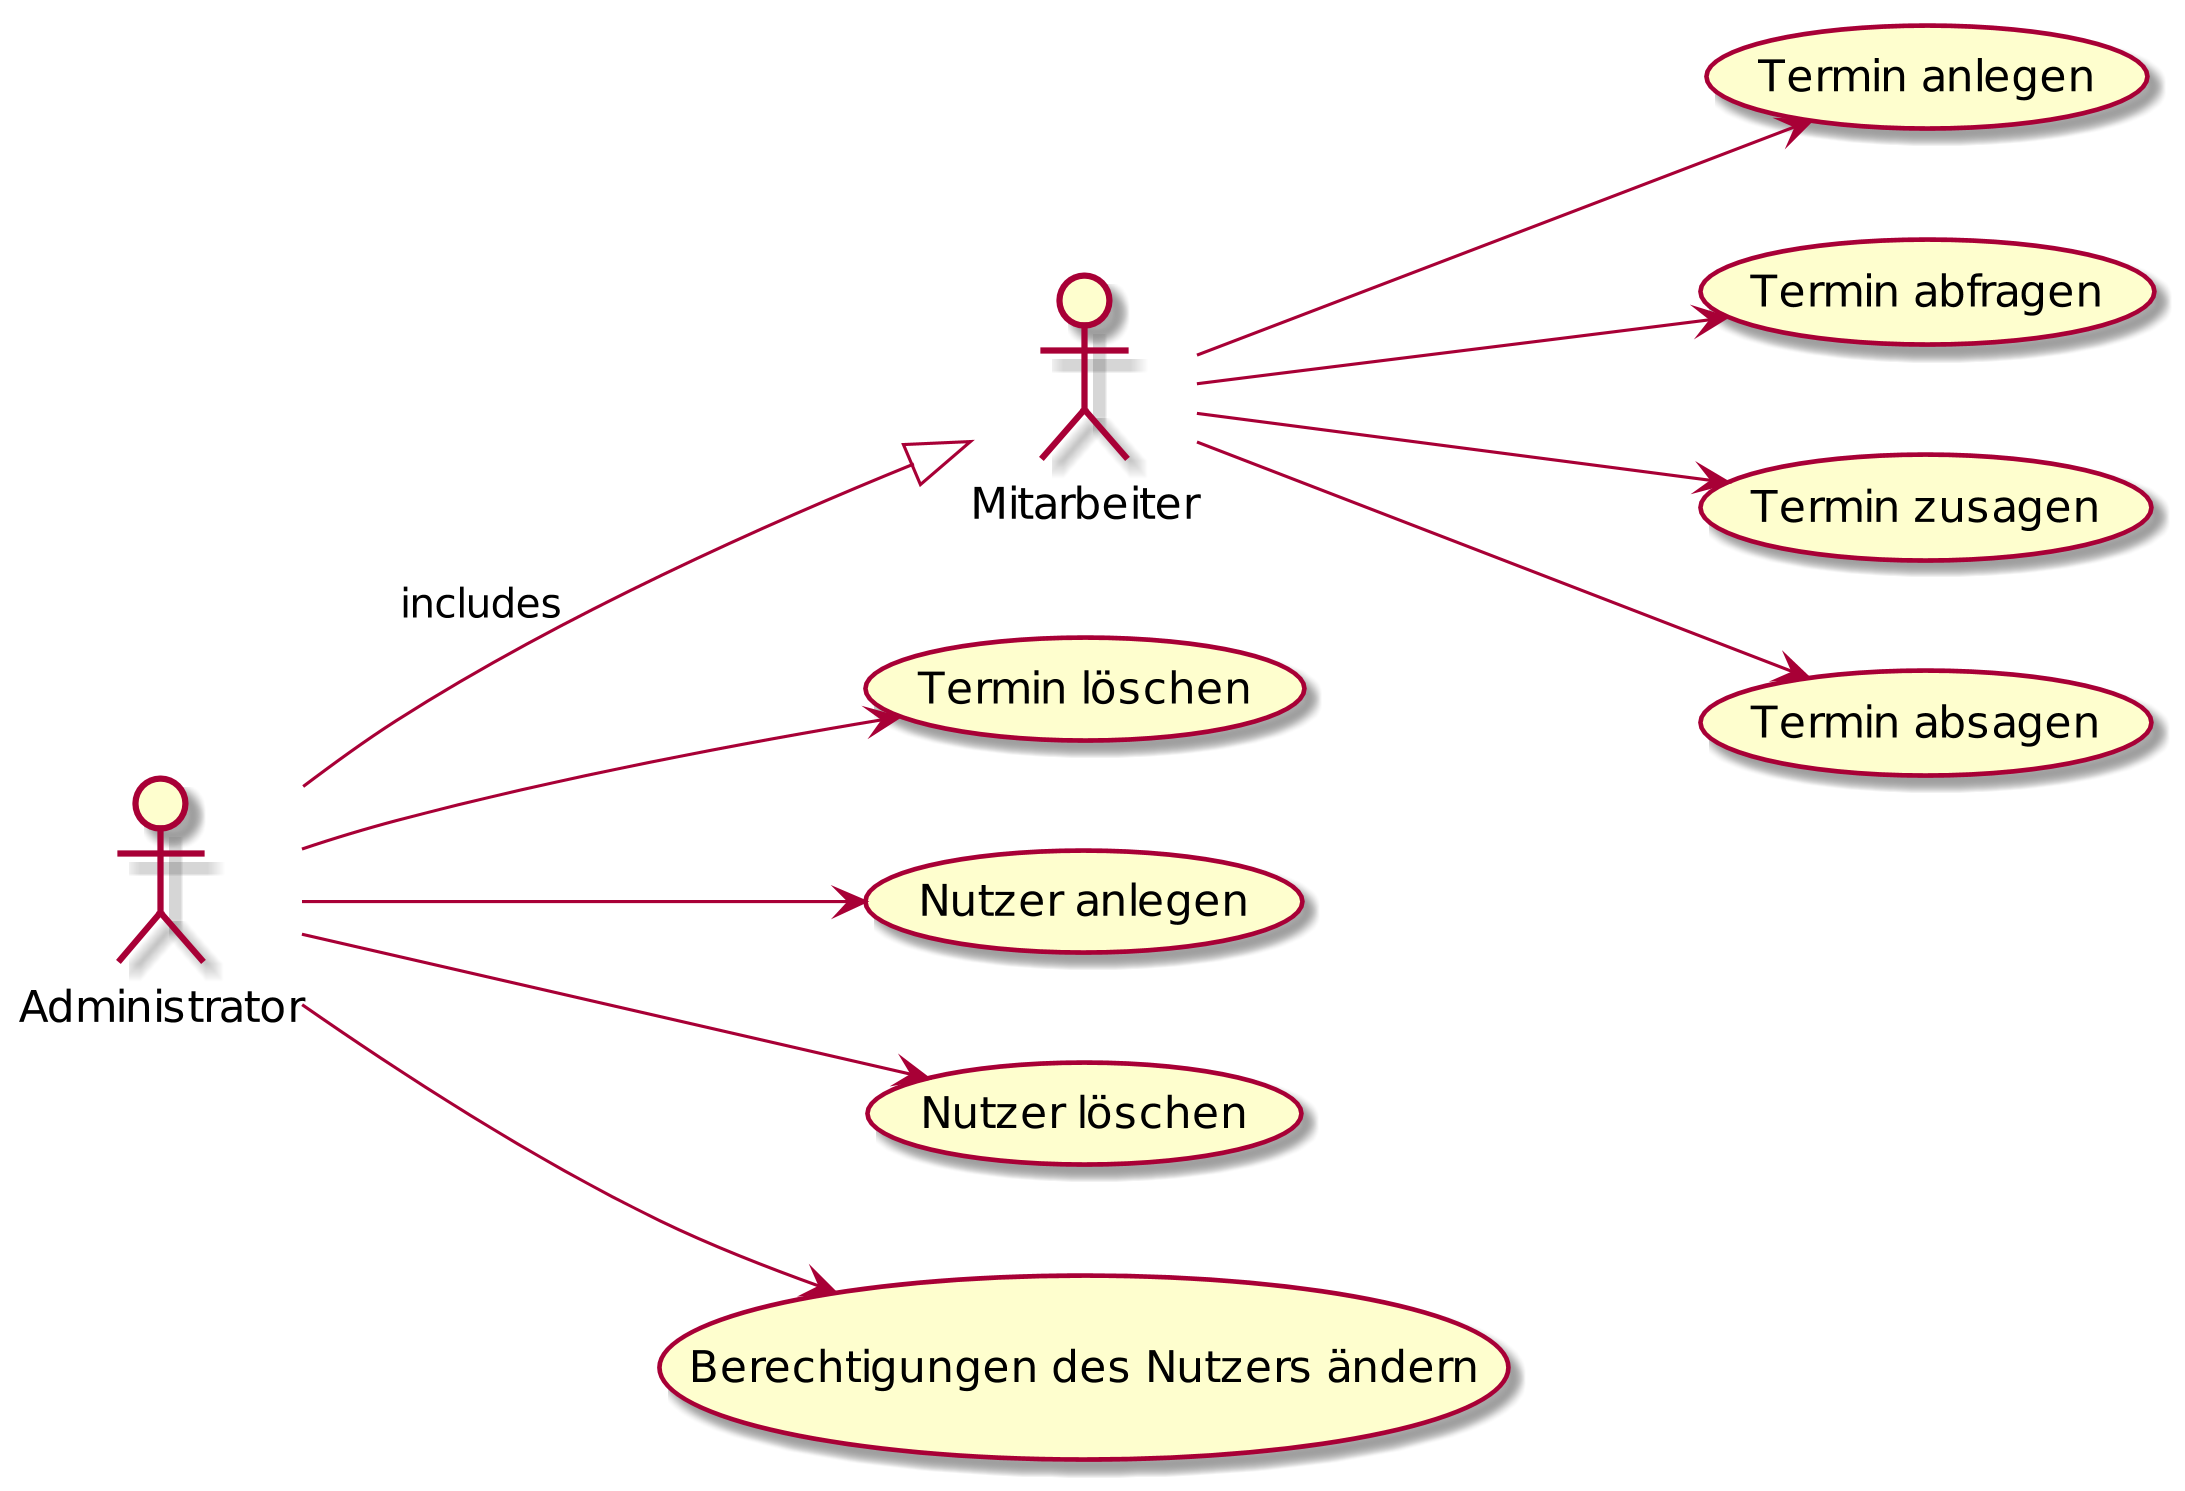
\includegraphics[width=0.9\textwidth]{../docs/uml/usecase-berechtigung.png}
    \caption{Anwendungsfalldiagramm zur Abgrenzung von Mitarbeiter und Administrator}
    \label{img:usecase-berechtigung}
\end{figure}
% Ferdi will, Ferdi verlangt, Ferdi lässt Spielraum (feine ziele)
% Festgelegte Begriffe, allgemeingültige Aussagen für das Dokument

\clearpage
\section{Auswahl eines Bot-Frameworks}
\label{botframework}

\subsection{Vergleichsparameter}
Für einen Vergleich der einzusetzenden Bot-Frameworks werden für diese im Folgenden Vergleichsparameter definiert. Dabei ist es wichtig, diese an den Anforderungen aus dem vorherigen Kapitel sowie technischen Aspekten zu orientieren.

Jeder Parameter muss folgende Kriterien erfüllen:

\begin{itemize}
    \item messbar, als Zahlen- Text- oder Wahrheitswert
    \item generisch, d.h. auf die zu vergleichenden Frameworks anwendbar
    \item nachweisbar, d.h. die Herkunft des Wertes ist nachvollziehbar
\end{itemize}

Aus \autoref{tab:botparameters} sind passende Bewertungsparameter gemäß der oben genannten Anforderungen zu entnehmen.

% evtl. booktabs statt tabularx
\begin{table}[htbp]
    \begin{tabularx}{\textwidth}{|l|X|p{6cm}|}
   \hline
   \textbf{Parameter} & \textbf{Beschreibung} & \textbf{Quelle} \\
   \hline
   Alter & Datum des ersten Commits im Master-branch & \verb+git log --reverse | head -3+\\
   \hline
   Aktivität & Commits in den Master-branch, Anz.\ Pull-Requests & GitHub Projektübersicht \\
   \hline
   Popularität & Anz.\ \enquote{Stars} und \enquote{Forks} & GitHub \\
    \hline
   Codequalität & Testabdeckung und Anz.\ Issues & GitHub, Tests vorhanden \\
   \hline
   Komplexität & Anz.\ Klassen, SLOC\footnote{Source Lines of Code}, Dateigröße \textbf{ohne Beispiele, externe Abhängigkeiten etc.} & \verb+du+, Code, \verb+git ls-files | xargs wc -l+ \\
   \hline
   Programmiersprache & primär verwendete Programmiersprache & GitHub-Seite \\
   \hline
   Integrationsgrad & Anz.\ bereits vorhandener Integrationen & Website, Dokumentation, npm \\
   \hline
   Erweiterbarkeit & Anz. der Erweiterungsmodule & Code, Dokumentation \\
   \hline
   Dokumentation & Dokumentation vorhanden ja/nein & docs-Ordner oder GitHub-Wiki \\
   \hline
   Lizenz & Art der Lizenz des Projektes & LICENSE.md im Git-Repositorium \\
   \hline
\end{tabularx}
\caption{Parameter zum Vergleich der Bot-Frameworks}
\label{tab:botparameters}
\end{table}

Die Aussagefähigkeit der in \autoref{tab:botparameters} enthaltenen Parameter ist stellenweise kritisch zu hinterfragen, da die Genauigkeit zugunsten der Generizität eingeschränkt wurde. 
Beispiele hierfür sind folgende:
\begin{itemize}
    \item Testabdeckung: je nach Auswahl und Integration der Testbibliothek kann die Testabdeckung immer 100\% betragen
\item SLOC: viele Codezeilen deuten nicht zwingend auf guten Code hin (von Kommentaren wird hier, per Definition, abgesehen)
\end{itemize}

Unter Beachtung der Einschränkungen und der Kombination aller Parameter ist eine differenzierte Gegenüberstellung durchführbar.

\subsection{Auswahl möglicher Frameworks}

Aufbauend auf den zu Beginn gestellten Anforderungen entfallen Frameworks:
\begin{itemize}
    \item deren Quelltext nicht frei verfügbar ist
    \item die eine dauerhafte Verbindung zum Hersteller benötigen
    \item die nicht kostenfrei sind
\end{itemize}

Durch diese Einschränkungen sind z.B. das von facebook entwickelte wit-Botframework (\url{https://wit.ai/}) und das von Microsoft entwickelte Bot-framework (\url{https://dev.botframework.com/}) nicht Teil weiterer Betrachtungen.
Eine weitere Gruppe von Botframeworks zeichnet sich durch eine (meist zwingende) Anbindung an eine Spracherkennung aus, die für den hier gewünschten Anwendungsfall nicht benötigt wird. Dadurch wird z.B. \url{api.ai} nicht Teil weiterer Betrachtungen sein.


Weitere Botframeworks sind unter \url{https://github.com/abdelhai/awesome-bots} aufgelistet. 
Von den dort aufgelisteten Frameworks entsprechen hier \textbf{Botkit} (\url{https://botkit.ai/}) und \textbf{Hubot} (\url{https://hubot.github.com/}) den Anforderungen.

\subsection{Vergleich der Frameworks}

\begin{table}[htbp]
    \centering
    \begin{tabularx}{\textwidth}{|l|X|X|}
        \hline
        \textbf{Parameter} & \textbf{Botkit} & \textbf{Hubot} \\
        \hline
        Alter (Stand 02.2018) & $\approx$ 2 Jahre & $\approx$ 5 Jahre \\
        \hline
        Aktivität & \makecell[l]{2078 Commits\\ 29 Pull-Requests} & \makecell[l]{2011 Commits\\ 5 Pull-Requests} \\
        \hline
        Popularität & \makecell[l]{7.813 Sterne\\ 1.714 Forks} & \makecell[l]{13.817 Sterne\\ 3.269 Forks} \\
        \hline
        Codequalität & \makecell[l]{115 Issues\\ Testabdeckung 100\%} & \makecell[l]{30 Issues\\ Testabdeckung 100\%} \\
        \hline
        Komplexität & 35259 SLOC & 7472 SLOC \\
        \hline
        Programmiersprache & TypeScript & CoffeeScript \\
        \hline
        Integrationsgrad & 12 & 62 \\
        \hline
        Erweiterbarkeit & 28 & $\approx$ 50 \\
        \hline
        Dokumentation & ja & ja \\
        \hline
        Lizenz & frei, MIT & frei, MIT \\
        \hline
    \end{tabularx}
    \caption{Vergleich von Botkit und Hubot}
    \label{tab:comparebotkithubot}
\end{table}

% Zwischenfazit: Botkit ist größer und umfangreicher, Hubot kleiner und simpler.
% Würde ich am Ende von TypeScript vs. CoffeeScript abhängig machen

Wie in \autoref{tab:comparebotkithubot} ersichtlich, bietet Hubot aufgrund der längeren Entwicklungszeit eine größere Anzahl von Nutzern und Integrationen. Des Weiteren ist Hubot auf die praktische Notwendigkeit bei GitHub zurückzuführen, die Entwicklungsprozesse an ChatOps\footnote{Ausführen von Deployment-Befehlen etc. direkt aus dem Chat-Programm, Hintergrund siehe: \url{https://www.youtube.com/watch?v=NST3u-GjjFw}} auszurichten.

Im Gegensatz dazu bietet Botkit flexiblere Einsatzmöglichkeiten und Integrationen in andere Dienste wie NLU\footnote{Natural language understanding}, Apps und Messenger. Aufgrund des relativ jungen Projektalters von zwei Jahren und der vergleichsweise höheren Anzahl an Bugtickets (\enquote{Issues}) und Codezeilen, wird die Codequalität Botkits geringer als die Hubots bewertet.

Beide Frameworks dienen dabei unterschiedlichen Zielen: während Botkit eher als Rahmenwerk für darauf aufbauende Bots anzusehen ist, ist der Bot als solches direkt bei Hubot integriert und kann modular erweitert werden. Da beide Frameworks unter MIT-Lizenz stehen und zu JavaScript kompilieren, sind diese aus lizenzrechtlicher und technischer Sicht für das Projekt \enquote{Steckerbot} geeignet.

Für den in \autoref{anforderungen} beschriebenen Einsatzzweck fällt die Entscheidung auf \textbf{Hubot}. Im Vergleich zu Botkit bewerten die Autoren Hubot als strukturell simpler und näher am Ziel der praktischen Slack-Integration ausgerichtet. Botkit erfüllt diese Anforderungen auch, hatte jedoch keine so lange Reifephase wie Hubot.

Im weiteren Verlauf dieses Dokuments werden deshalb \enquote{Hubot}, \enquote{Botframework} und \enquote{Bot} synonym verwendet.


% HuBot, BotKit
% Einschränkungen der Auswahl weil ...

\clearpage
\section{Entwurf eines Modells}
\subsection{Anforderungsanalyse mittels Use-Case-Betrachtung}
% TODO: Struktur der Überschriften ändern, diese hat nur einen 
% Unterpunkt und passt thematisch nicht

\subsubsection{Interaktion über Slack}

Es werden folgende Befehle für die Interaktion definiert.

\begin{table}[H]
\centering
\begin{tabular}{l|l}
  Befehl & Bedeutung \\
 \hline
% für vergessliche Leute
 zeige Schicht & zeigt die nächste Schicht für die aufrufende Person an \\
 zeige Schichten & zeigt alle zukünftigen Schichten für die aufrufende Person an \\
 zeige alle Schichten & zeigt einen Schichtplan an, welcher alle Mitglieder enthält \\
 
% jedes Mitglied muss pro Jahr mindestens x mal an die Bar
 zeige Anzahl Schichten & zeigt die geleisteten Schichten für dieses Jahr an \\
 zeige Anzahl alte Schichten & zeigt die geleisteten Sichten für letztes Jahr an \\
 
% zum Anzeigen der Auswahl an welchen man teilnehmen  möchte
 zeige Termine & zeigt alle kommenden Termine $t_i$ an \\
 zeige Veranstaltungen & zeigt alle zukünftigen Veranstaltungen $v_i$ an ($V \subseteq T$) \\
 zeige Sitzungen & zeigt alle zukünftigen Sitzungen $s_i$ an ($S \subseteq T$) \\
 
% für Termin eintragen
 nehme Teil an $t_i$ & trägt den aufrufenden Nutzer als Teilnehmer für $t_i$ ein \\
 nehme nicht Teil an $t_i$ & trägt den aufrufenden Nutzer für $t_i$ aus\\

 % Utilities
 hilf mir & zeigt alle verfügbaren Kommandos an \\
 Danke & bricht die aktuelle Konversation ab
 
 wann ist der nächste termin?
 trag mich ein
 
 
\end{tabular}
\caption{Befehle zur Chatbotinteraktion}
\label{tab:chatbotinteraktion}
\end{table}

Die Befehle in \autoref{tab:chatbotinteraktion} folgen einem vereinfachtem Schema natürlicher Sprache: $<Prädikat (Imperativ)> <Subjekt>$. Die Struktur der Befehle soll dabei einfach zu merken, auf menschlicher Sprache basierend und auch auf mobilen Geräten mit wenig Tipparbeit verwendbar sein. Bei einem optionalen Einsatz einer Spracherkennung sind auch komplexere Satzkonstruktionen möglich, für den hier zu erfüllenden Zweck genügt das Schema aus $<Befehl> <Objekt> <Filter>$. Wie in \cite{ZueConversationalinterfacesadvances2000} beschrieben, weicht die Art der Kommunikation von Mensch-zu-Mensch und Mensch-zu-Bot voneinander ab, worauf bei der Definition der Interaktionsbefehle geachtet wurde. Es ist nach Ansicht der Autoren wenig sinnvoll, einen Bot zu entwickeln, der durch den Zugriff auf große Datenmengen den Eindruck von Intelligenz vermittelt, die aber durch ihre Begrenzung dem Nutzer keinen Mehrwert bietet. Der hier entwickelte Bot verfügt bewusst über ein begrenztes Vokabular, so dass er nur die vom Nutzer gewünschten Informationen liefert; die Kenntnis der Befehle obliegt dem Nutzer.

Aus den in \autoref{tab:chatbotinteraktion} definierten Befehlen wurden die Aktivitätsdiagramme \autoref{img:activity-zeige} und \autoref{img:activity-teilnahme} erstellt, um die Reihenfolge der Interaktion besser zu strukturieren.

\begin{figure}[htbp]
    \centering
    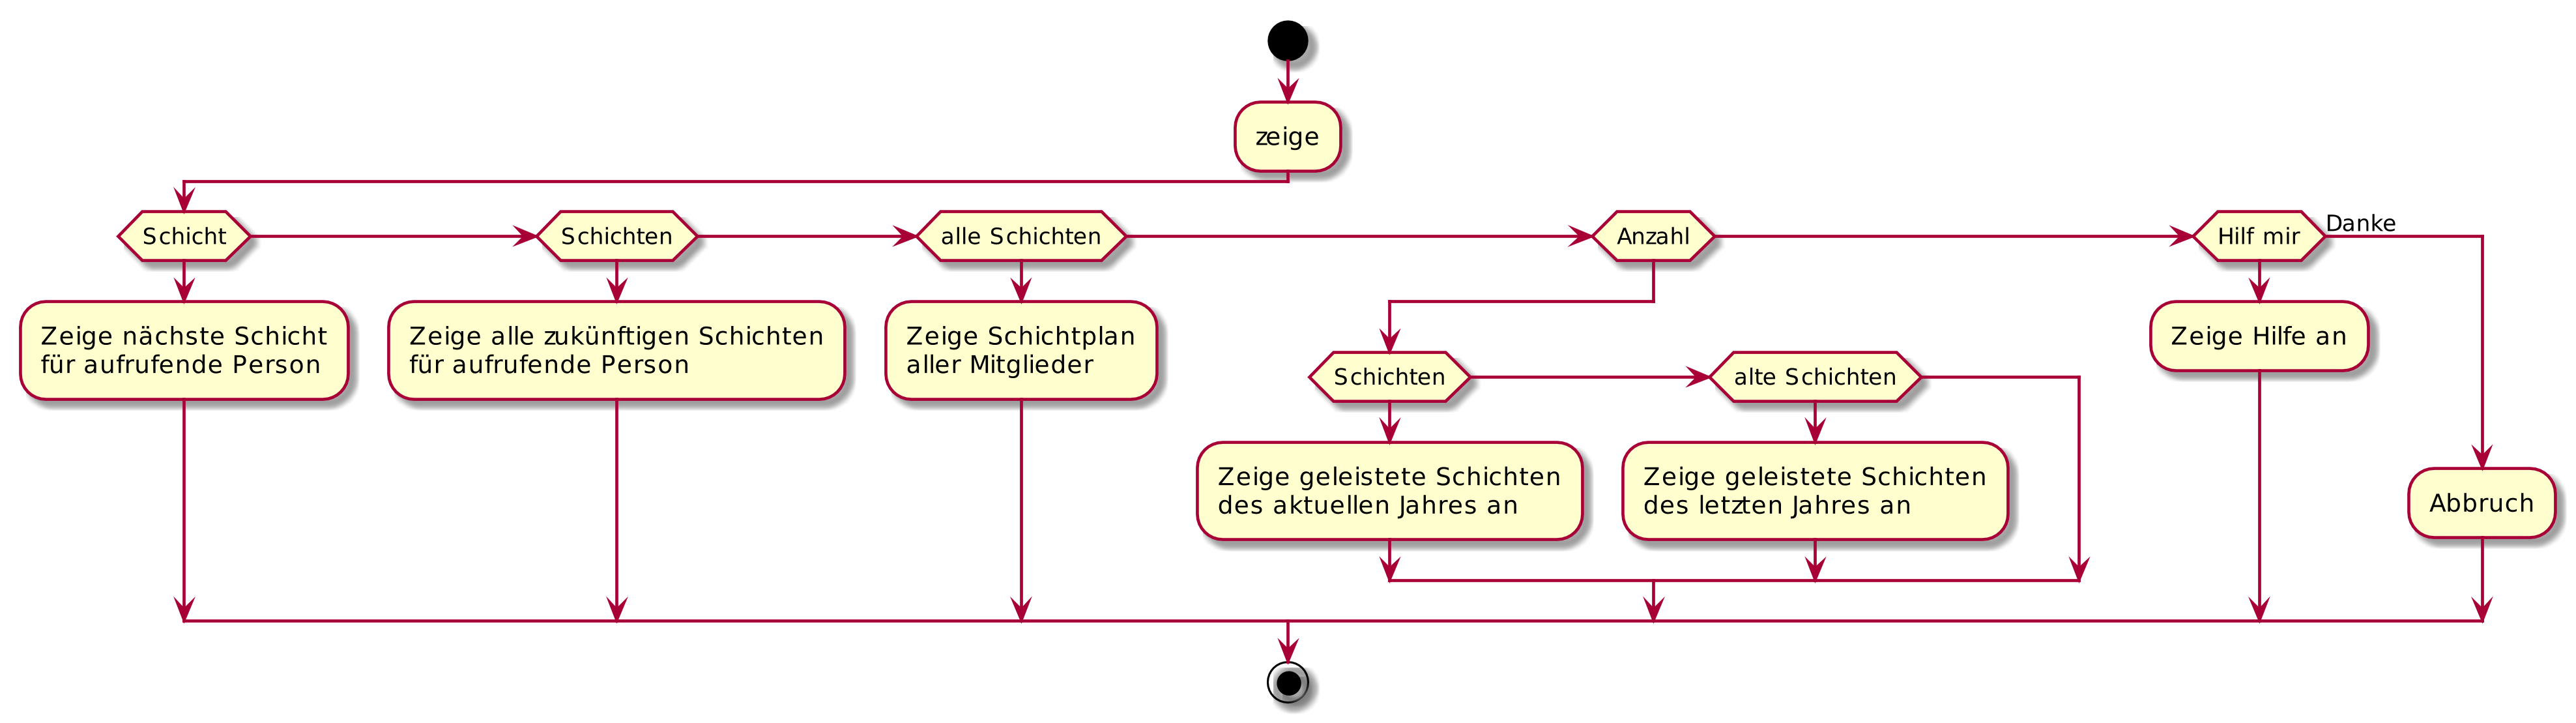
\includegraphics[width=\textwidth]{../docs/uml/activity-zeige.png}
    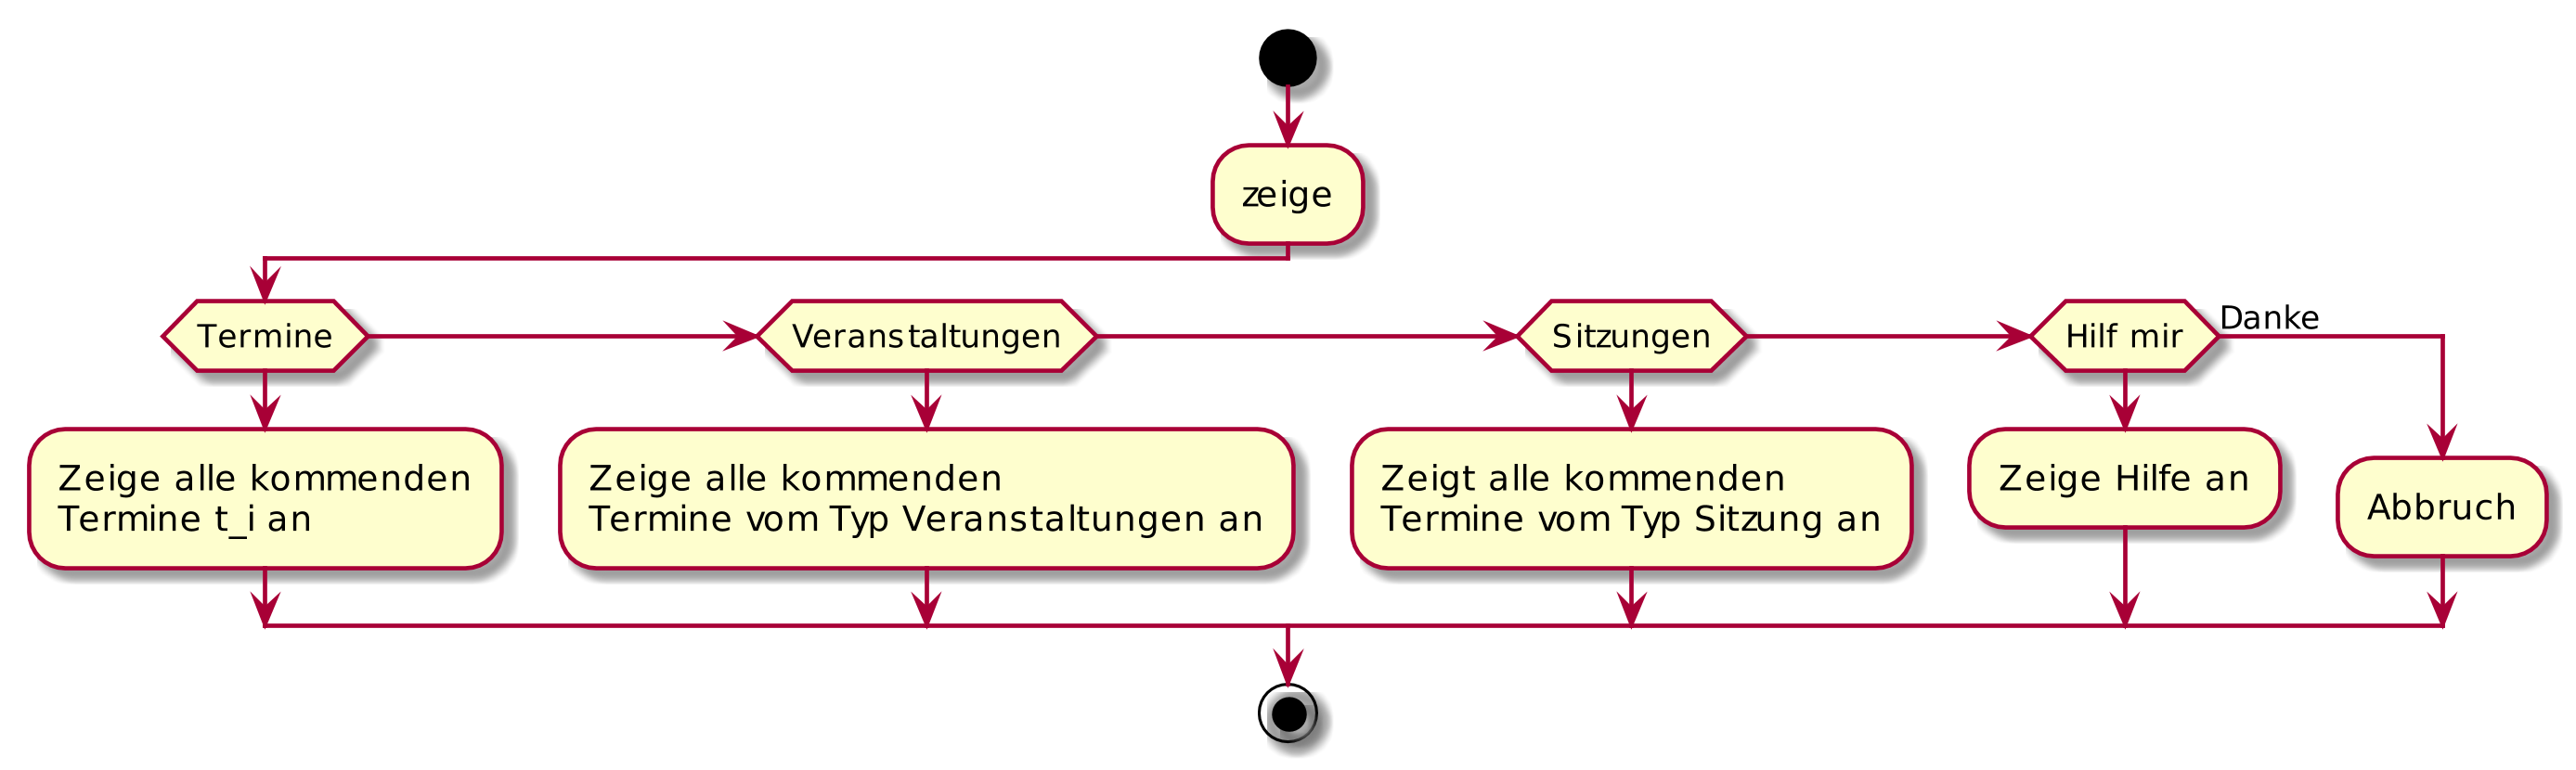
\includegraphics[width=0.9\textwidth]{../docs/uml/activity-zeige2.png}
    \caption{Aktivitätsdiagramme zum Anzeigen von Terminen}
    \label{img:activity-zeige}
\end{figure}

\begin{figure}[htbp]
    \centering
    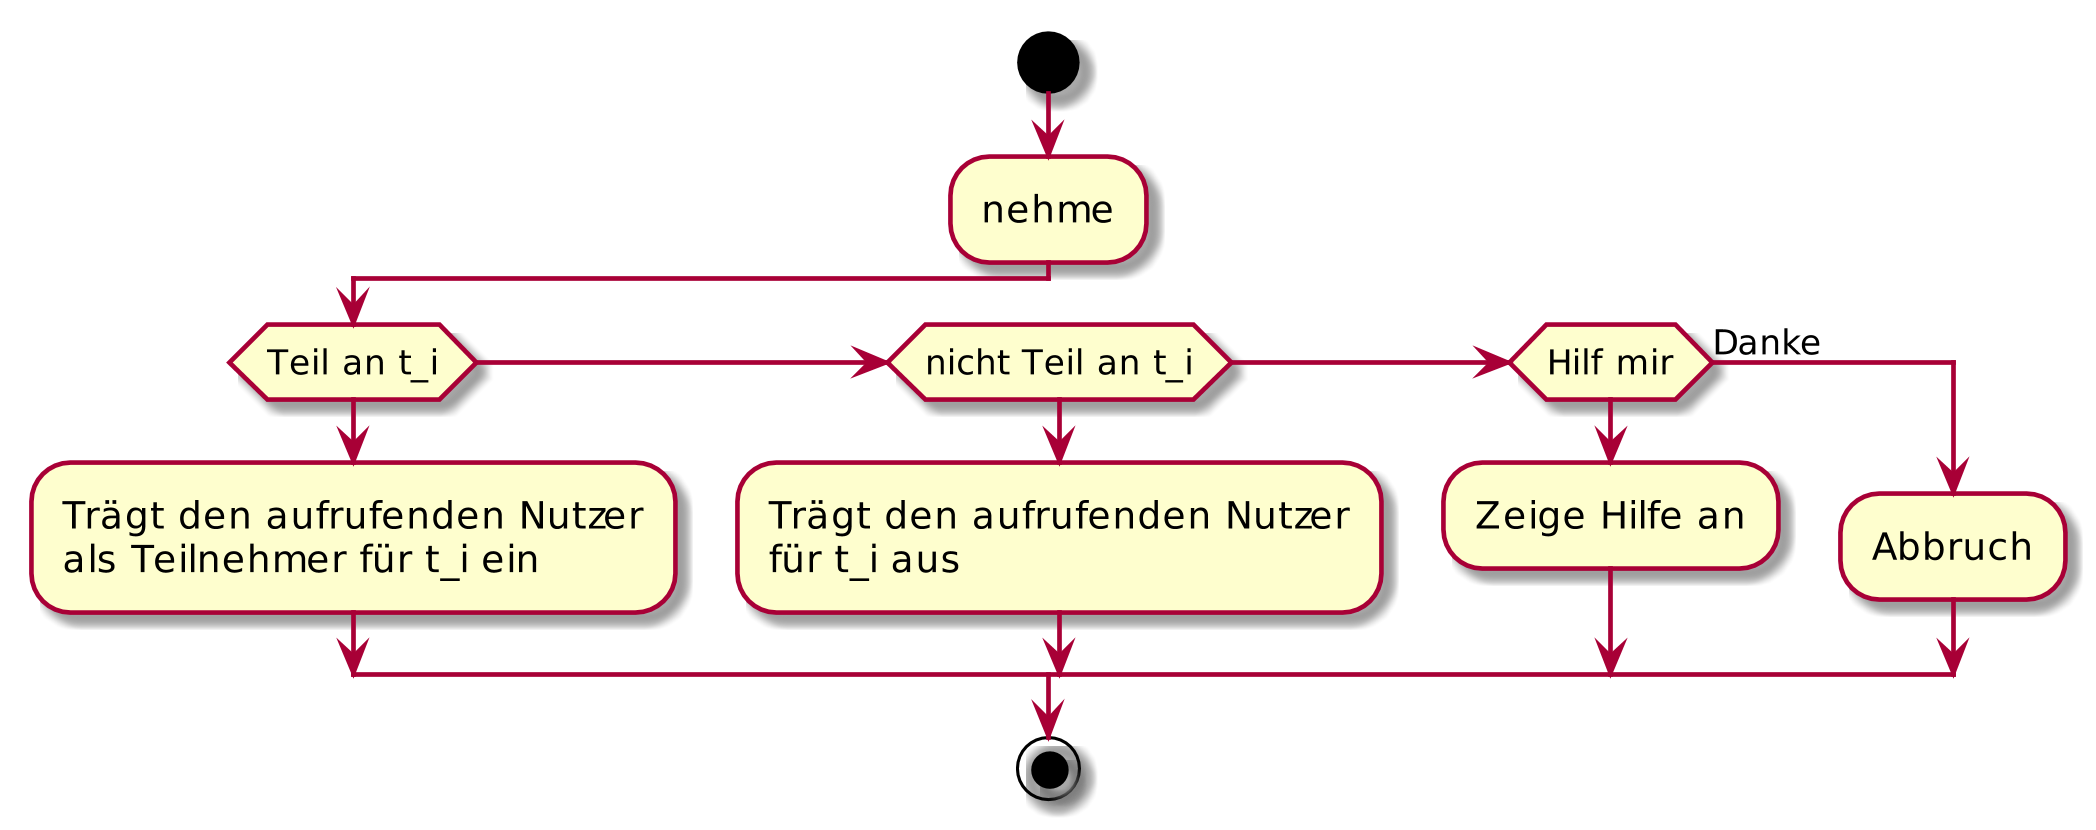
\includegraphics[width=0.7\textwidth]{../docs/uml/activity-teilnahme.png}
    \caption{Aktivitätsdiagramm zur Teilnahme an Terminen}
    \label{img:activity-teilnahme}
\end{figure}


\subsection{Datenbankschema}

Das Datenbankschema soll laut Anforderung unabhängig von einem spezifischen Chatbot nutzbar sein. Falls ein Chatbot ausgetauscht oder andere Interaktionsmethoden hinzugefügt werden, darf die Datenbank entsprechend keine Abhängigkeiten besitzen. Es wird deshalb ein Datenbankschema angelegt, welches nur die Terminverwaltung abbildet und anschließend eine Erweiterung hinzugefügt, welche die notwendigen Schlüssel auf die verwendete Plattform abbildet.

% Hier das DB-Schmea rein und eine Fremdschlüsseltabelle für die Slack-Nutzernamen und bla

\begin{figure}[htbp]
    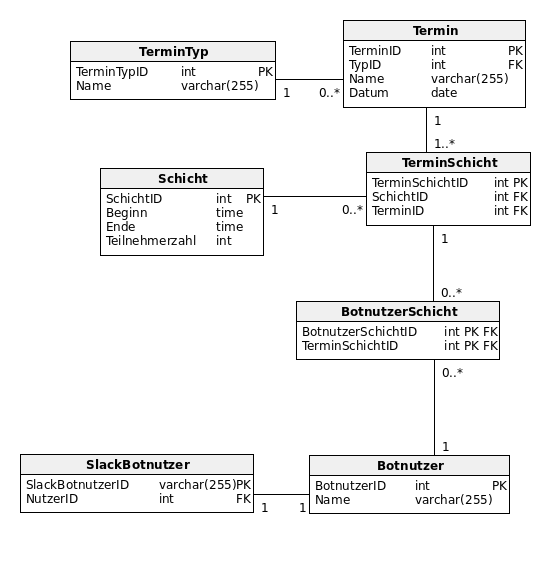
\includegraphics[width=\textwidth]{../docs/uml/Steckerbot-DB.png}
    \caption{Schema für die Termin-DB}
    \label{img:db-schema}
\end{figure}


\subsection{Kommunikationsschnittstellen}

Die kommunikation zwischen der Datenbank und dem Chatbot erfolgt auf dem gleichen Host, weshalb keine besonderen Fälle beachtet werden müssen. Der Kommunikationspfad zwischen dem Chatbot und Slack wird jedoch über ein Hochschulnetzwerk durchgeführt. In diesem sind in das Netzwerk des Clubs nur die Ports 80 und 443 freigegeben. Ausgehend ????????????????? doppeltes NAT aber Webseiten ok

Aus diesem Grund muss der Chatbot sich als Client mit Slack verbinden und darf keine Serveranwendung sein, welche ein Polling implementiert.

% vllt Grafik einfügen?


TODO: ERWEITERN
Slack hat eine option globale UIDs zum bot durchzuleiten. nützlich, wenn mehrere Workspaces genutzt werden - ist das der fall? ferdi fragen.

% Kommunikationspfade, Blockdiagramme, UML
% Datenhaltung, Datentransport, Sicherheit, Zukunftssicherheit, Austauschbarkeit, Robustheit, Erweiterbarkeit

\clearpage
\section{Realisierung des Modells}
% Warum welche Sprache
% Warum Abkürzungen im ggs zu Modell genommen
% Welche praktischen Hürden überwunden

\clearpage
\section{Analyse}
% Alle Anforderungen erfüllt?
% Wie gemessen?
% Blockdiagramme, MSCs, Fehlerbetrachtung
% Performance - Latenz?

\clearpage
\section{Fazit}
% Funzt? Jo
% Was wurde erledigt, was ¬ und warum?

\clearpage
\section{Aussicht}
% Empfehlungen für Verbesserungen, Erweiterungsmöglichkeiten, ...

\clearpage
\section{Benutzung des Endprodukts}
% Wo Daten eingeben, Wie per Hand testen, Wie Komponenten verbinden, (minimal) Beispiel


%Literatur
\nocite{GitHubGettingStartedHubot}
\nocite{BotkitBotkitToolkitbuilding}
\nocite{SlackConversationsAPI}

% % % % % % % % % % % % % % % % % % % % % % % % % INHALT

\newpage
\begin{appendices}
\section{Erstellung der Datenbank}
%TODO: Name aus Termin-Tabelle nehmen
\lstinputlisting[language=sql, caption={Erstellung der DB}, label=lst:promise]{code/SteckerbotDBModelcreate.sql}
\section{Anwendungsfalldiagramme}
\label{sec:usecase-diagram}

\begin{figure}[htbp]
    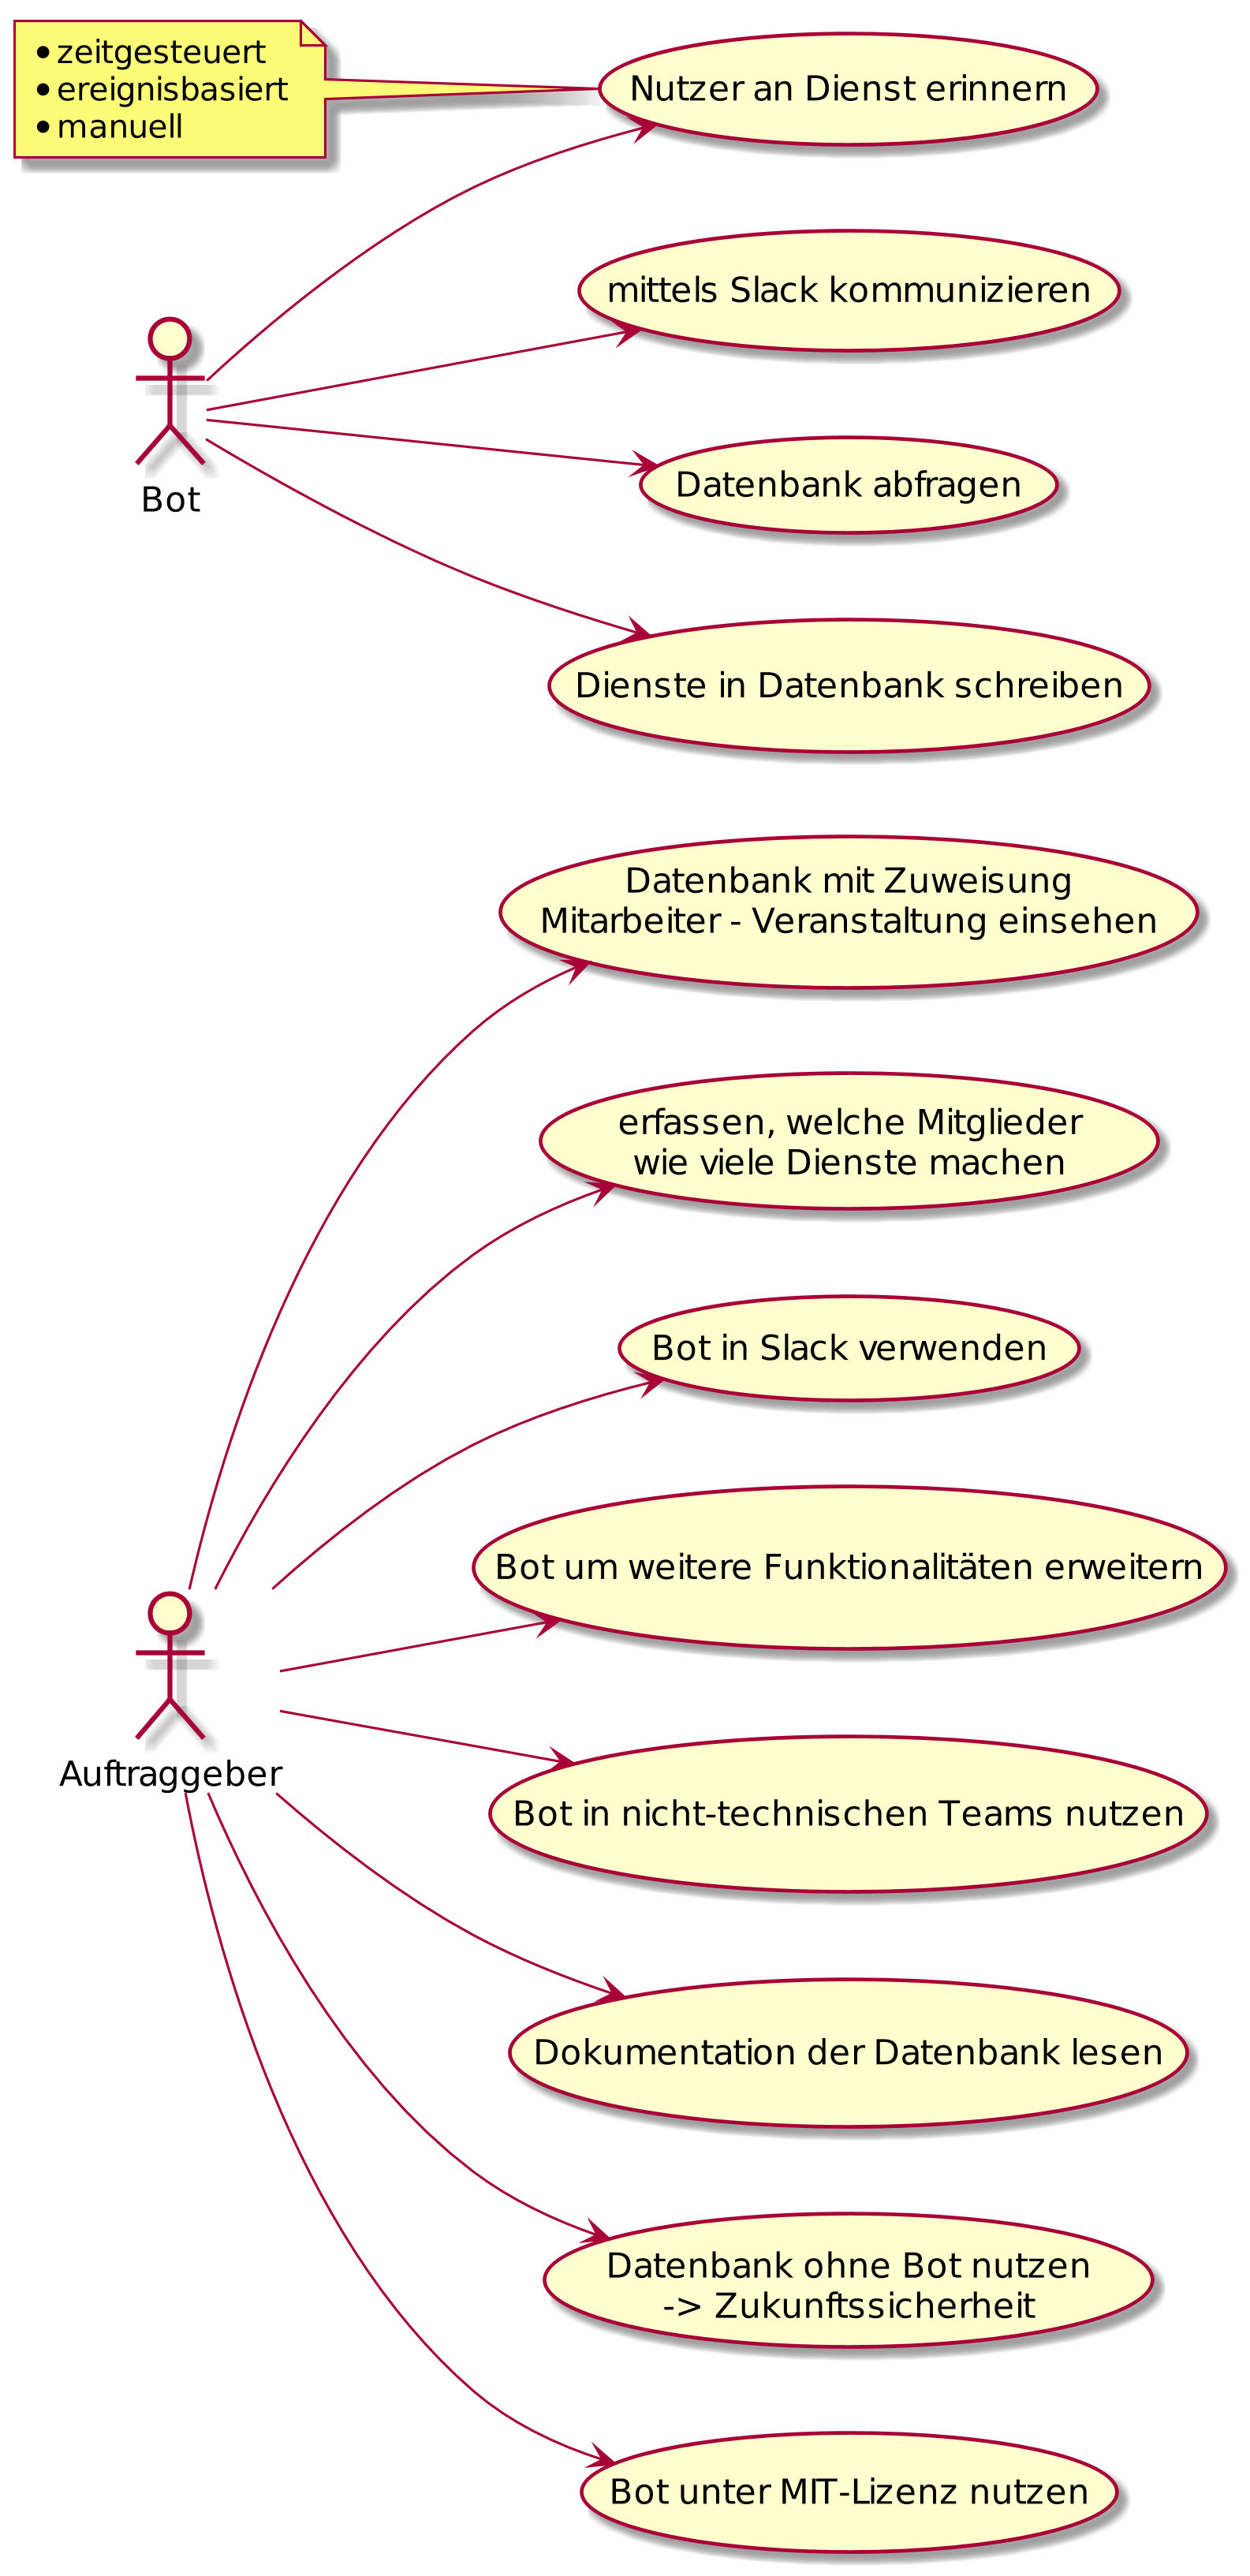
\includegraphics[width=0.7\textwidth]{../docs/uml/usecase-stakeholder.png}
    \caption{Anwendungsfalldiagramm für Auftraggeber und Bot}
    \label{img:usecase-auftrag}
\end{figure}

\begin{figure}[htbp]
    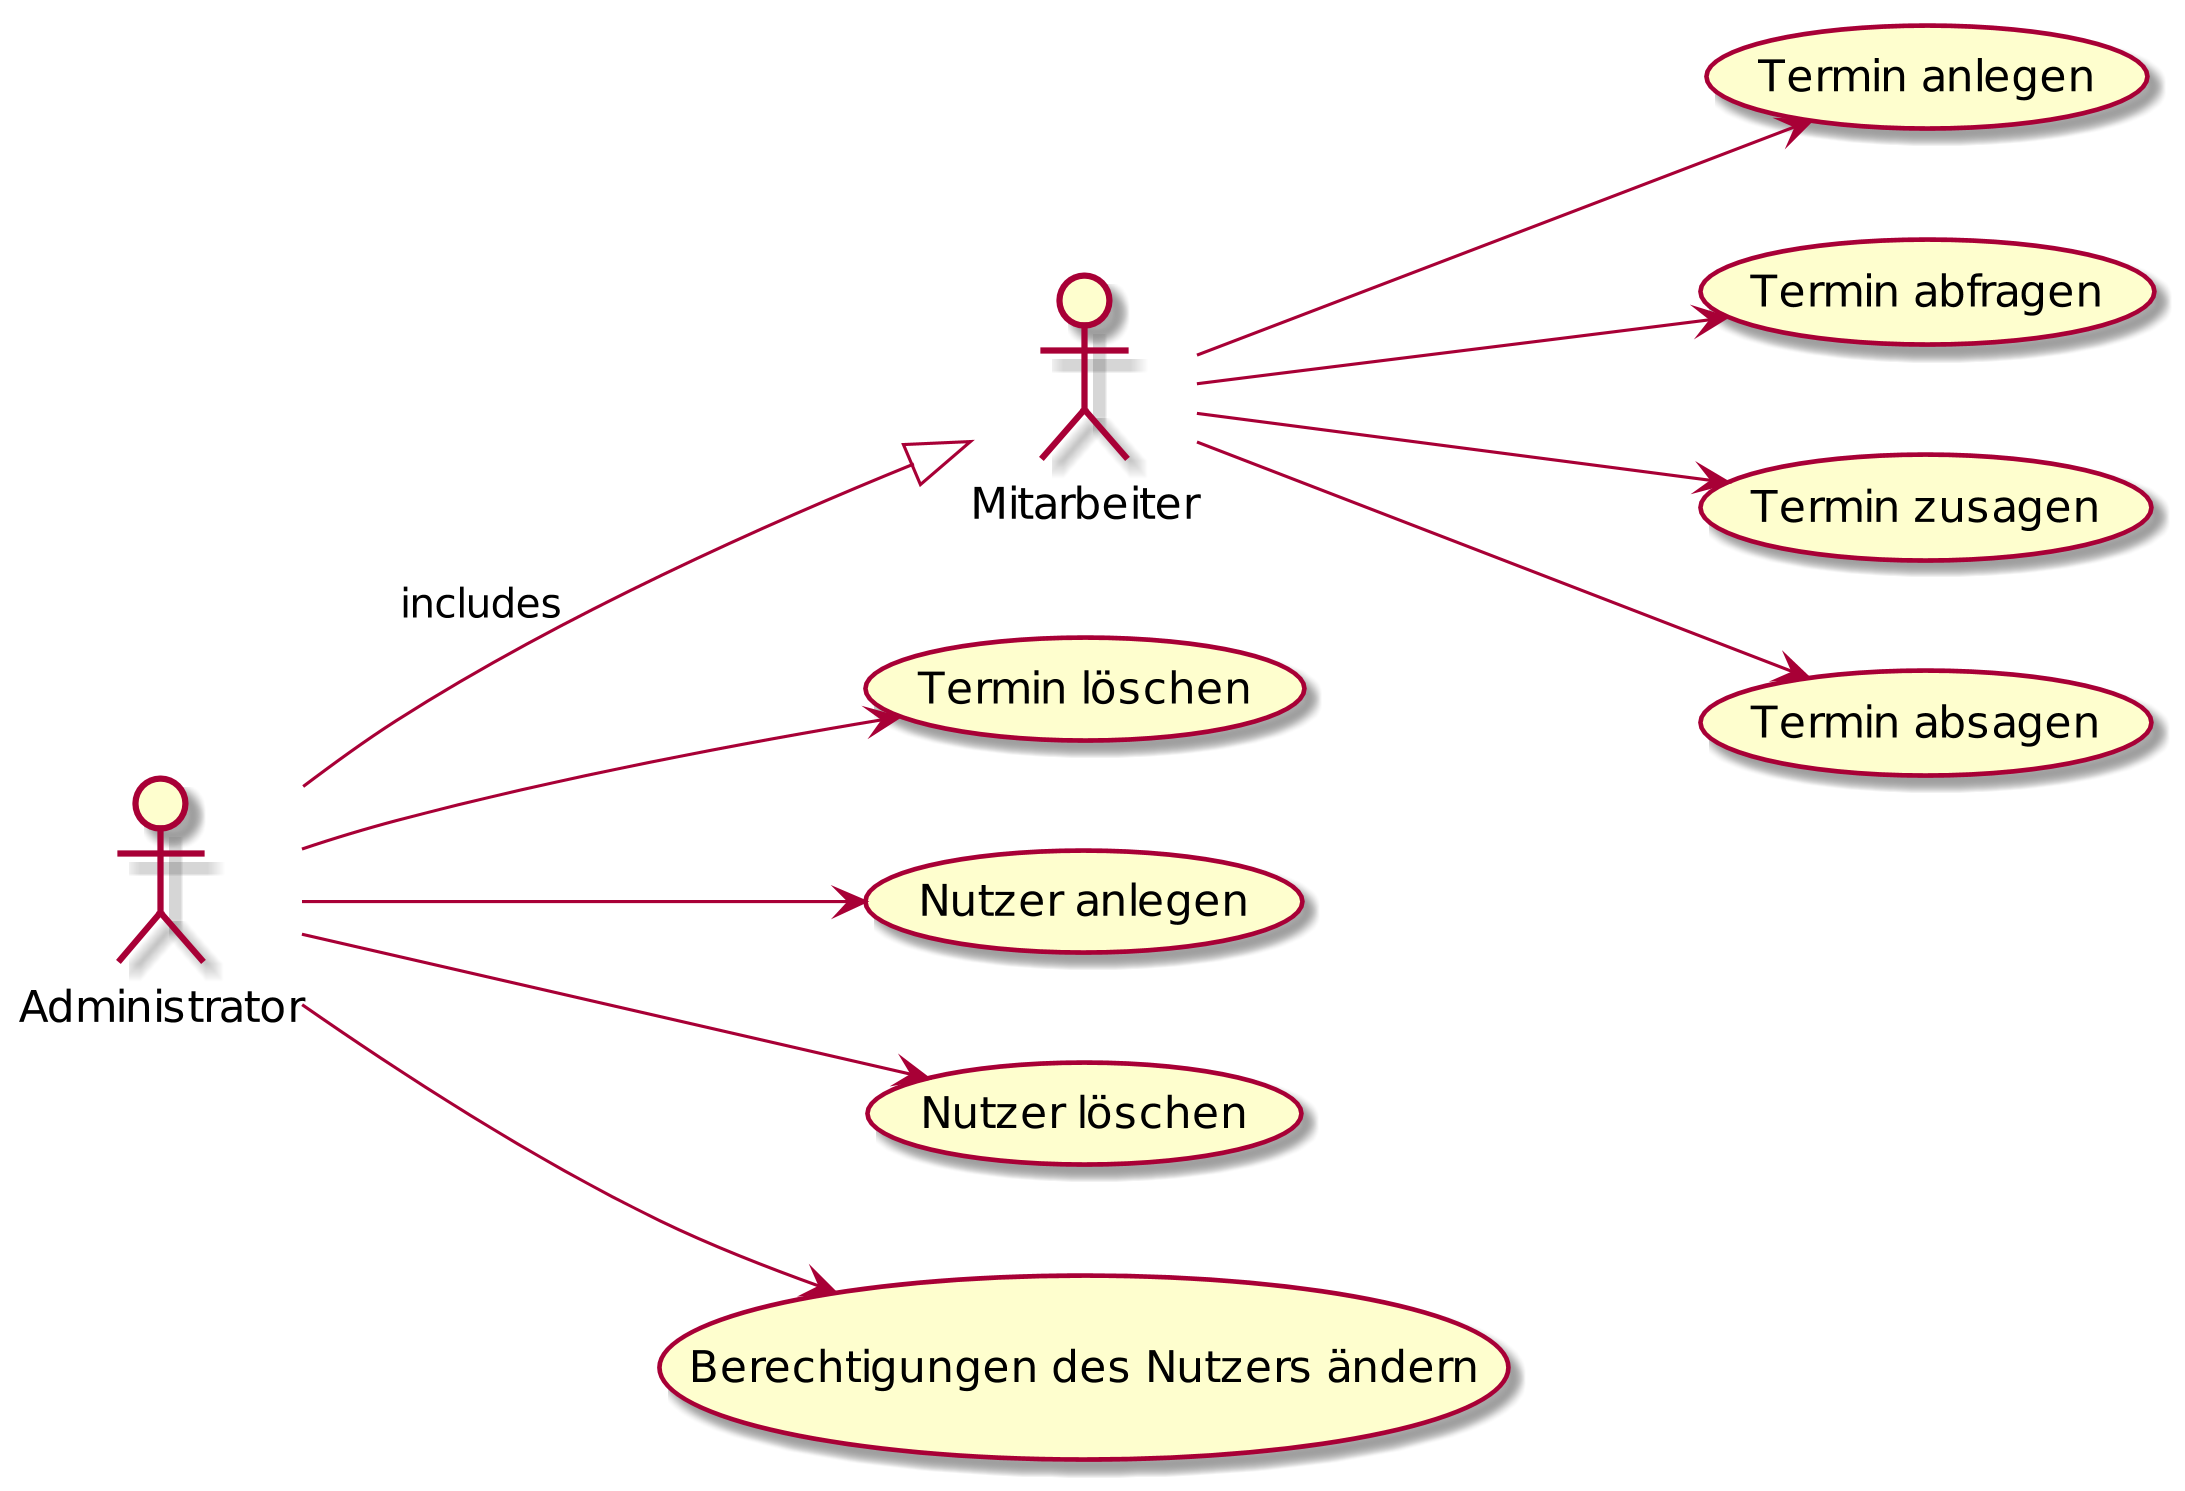
\includegraphics[width=0.9\textwidth]{../docs/uml/usecase-berechtigung.png}
    \caption{Anwendungsfalldiagramm zur Abgrenzung von Mitarbeiter und Administrator}
    \label{img:usecase-berechtigung}
\end{figure}

\section{Docker-Umgebung}
\lstinputlisting[language=bash, caption={Dockerfile für Hubot}, label=lst:dockerfile]{code/Dockerfile}
\lstinputlisting[language=yaml, caption={docker-compose.yml}, label=lst:docker-compose]{code/docker-compose.yml}

% \todo{Projektplan dazu?}
\section{Projektplan}
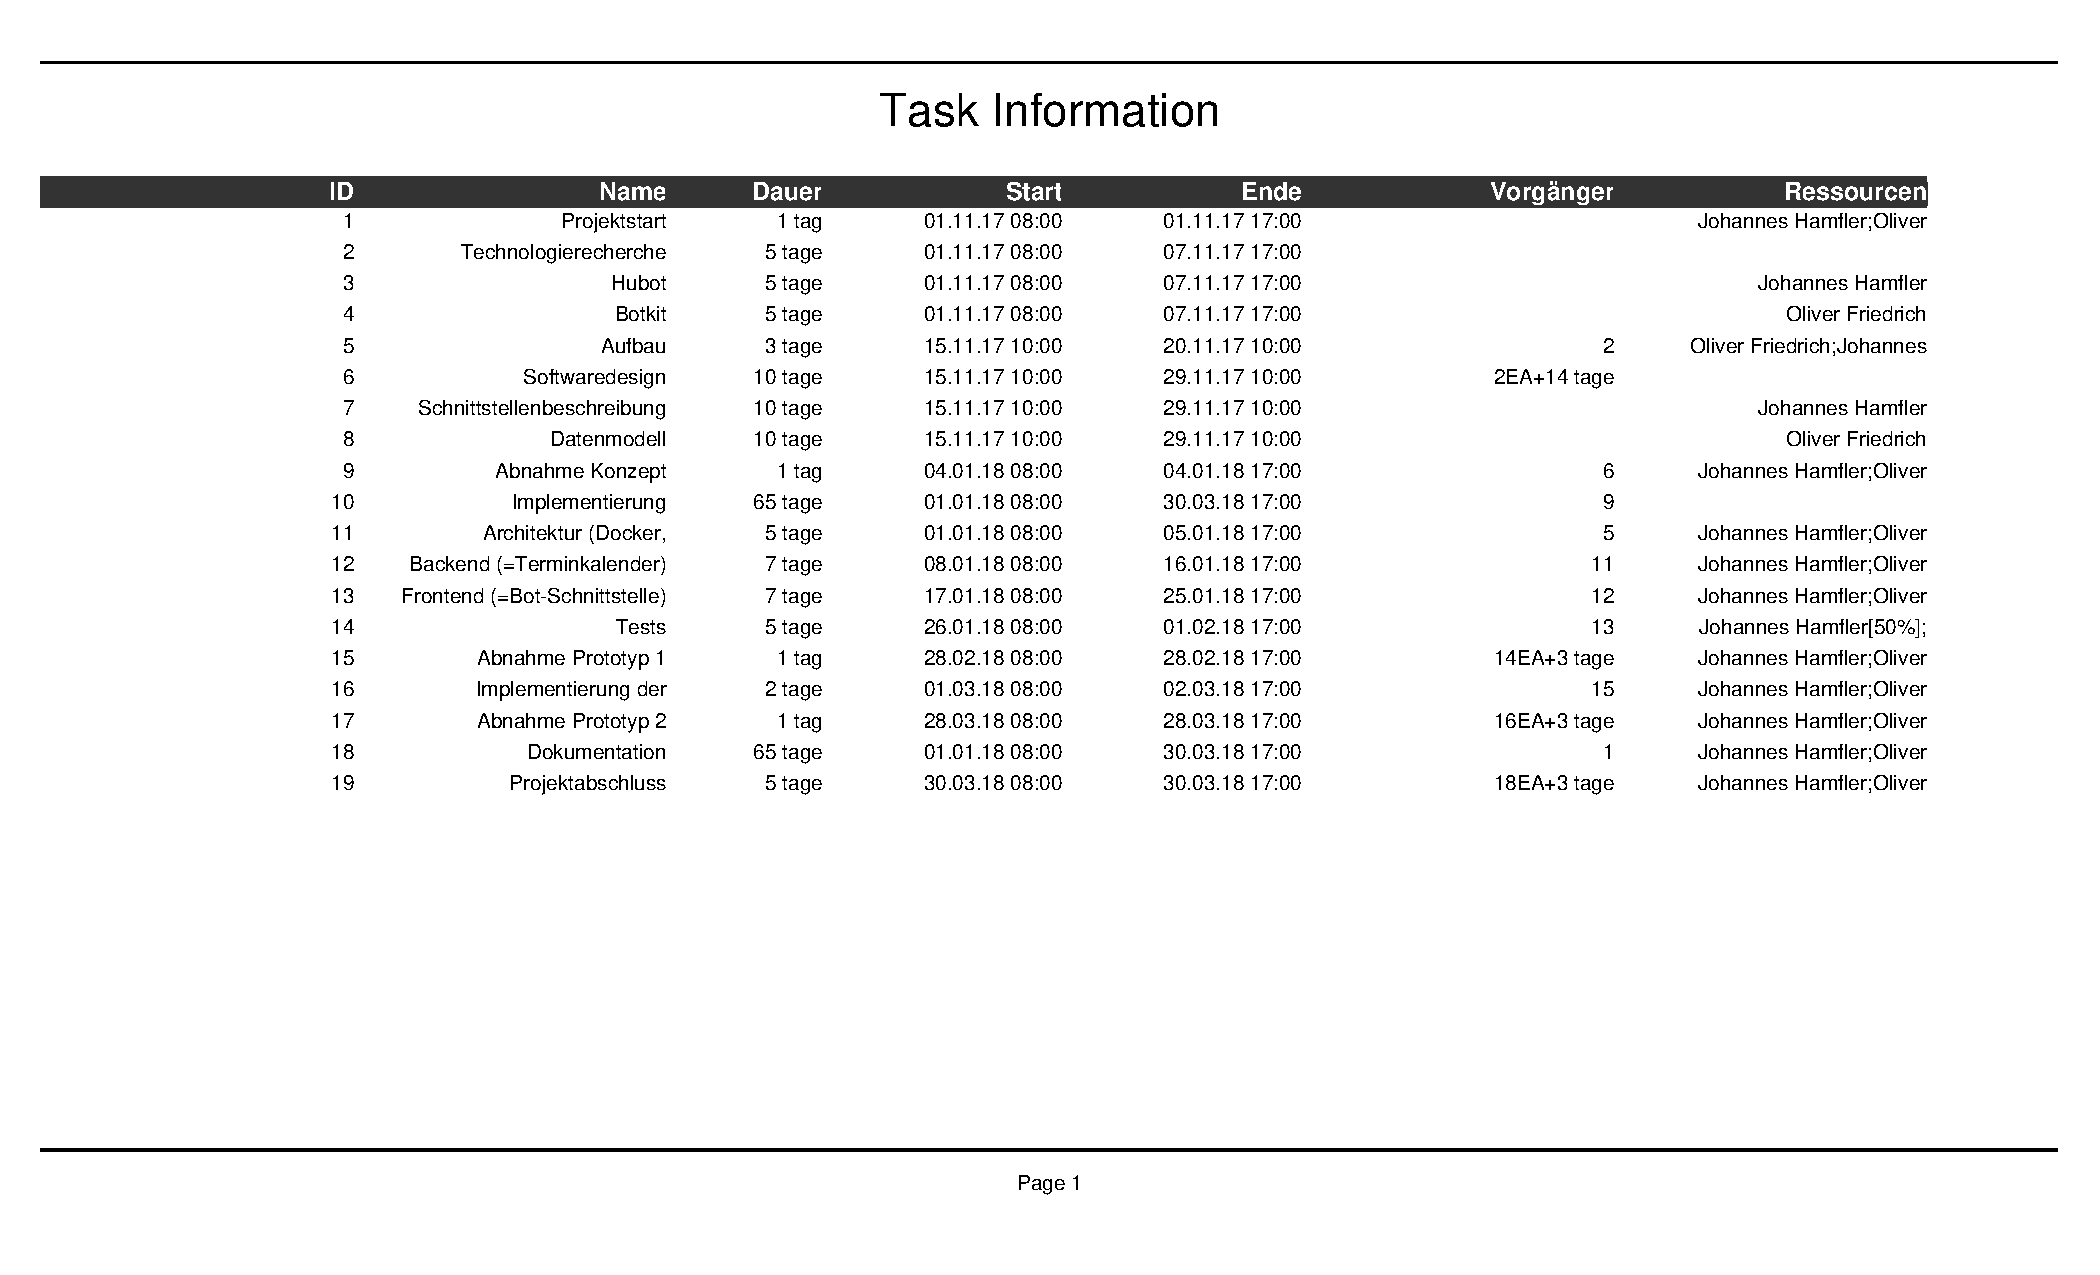
\includepdf[fitpaper]{../docs/Steckerbot_taskinfo.pdf}
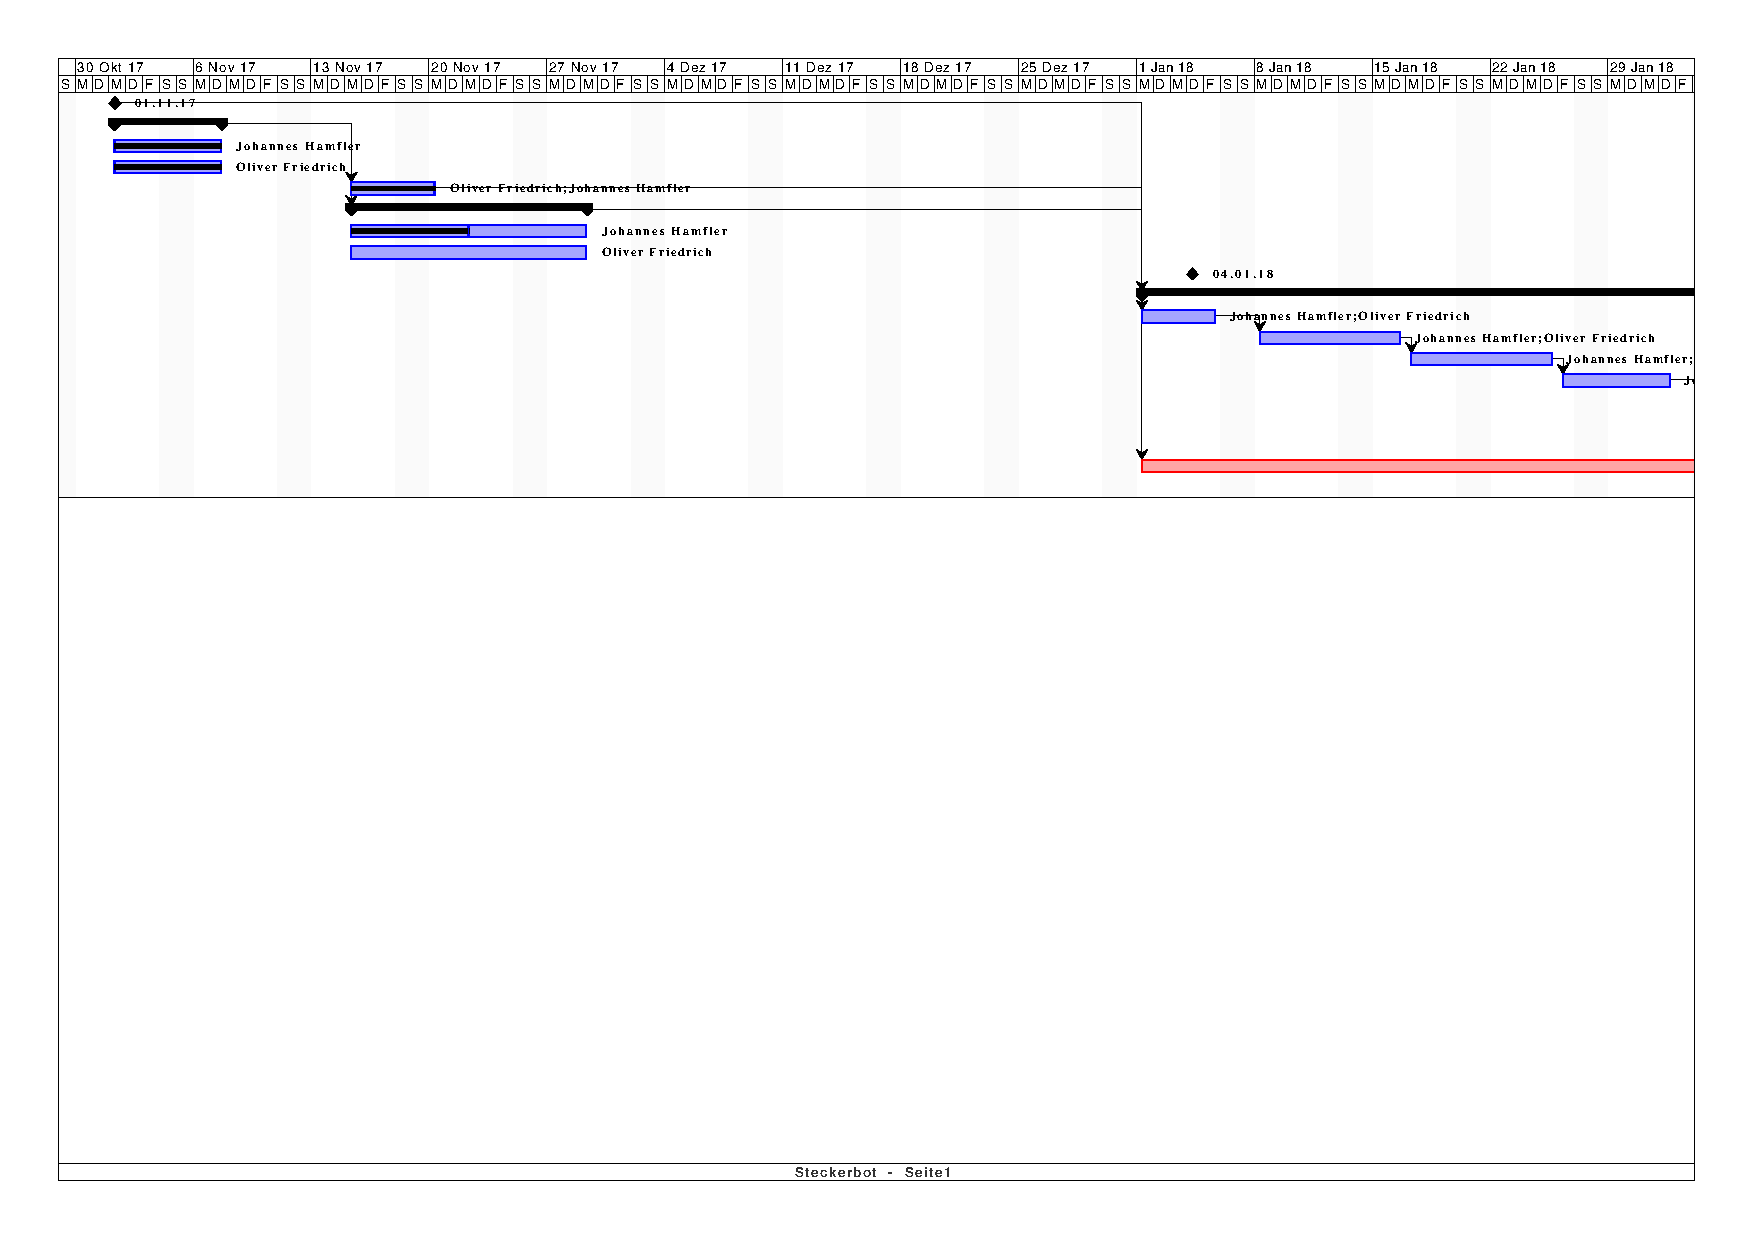
\includepdf[fitpaper]{../docs/Steckerbot_ganttchart.pdf}

\end{appendices}

\appendix


%Literatur
% \nocite{heap_ansible:_2016}
\newpage
%\lhead{{\footnotesize \textsc{Quellenverzeichnis}}}
\renewcommand\refname{Quellenverzeichnis}
\printbibliography%

\clearpage

%Abkürzungen ausgeben
%\deftranslation[to=German]{Acronyms}{Abkürzungsverzeichnis}
%\printglossary[type=\acronymtype,style=long,title=Abkürzungsverzeichnis]

%\lstlistoflistings
%\listoffigures


\setcounter{secnumdepth}{0}
\pagebreak
\ihead{\footnotesize \textsc{Selbständigkeitserklärung}}
\ohead{}
\section{Selbständigkeitserklärung}
\large
Hiermit erklären wir, dass wir die vorliegende Ausarbeitung selbständig verfasst und keine anderen als die angegebenen Hilfsmittel benutzt haben.
Die Stellen der Hausarbeit, die anderen Quellen im Wortlaut oder dem Sinn nach entnommen wurden, sind durch Angaben der Herkunft kenntlich gemacht. Dies gilt auch für Zeichnungen, Skizzen, bildliche Darstellungen sowie für Quellen aus dem Internet.

\vspace{3cm}
\unterschriftenfelder{Leipzig}{\firstAuthor}{\secondAuthor}

\end{document}
